\documentclass[conference]{IEEEtran}

\usepackage{amsmath}
\usepackage{amssymb}
\usepackage{bm}
\usepackage{graphicx}
\usepackage{booktabs}
\usepackage{multirow}
\usepackage{cite}
\usepackage{url}
\usepackage{siunitx}
\usepackage{xcolor}
\usepackage{hyperref}

\begin{document}

\title{
Vision-Based Closed-Loop Autonomous Spacecraft
Rendezvous with Robust Relative Pose Estimation
}

\author{
\IEEEauthorblockN{Bishwaswarup Nayak}
\IEEEauthorblockA{
Indian Institute of Science\\
Bengaluru, India\\
bishwaswarup@iisc.ac.in
}
}

\maketitle

% -------------------------------------------------
% Abstract
% -------------------------------------------------

\begin{abstract}
In this paper we present a simulation based visual navigation and guidance architecture to carry out on orbit autonomous rendezvous and proximity operations. The architecture uses HCW/J2 dynamics, analytically derived spacecraft feature landmark geometries, monocular perspective projection, RANSAC--EPnP pose estimation, a Multiplicative Extended Kalman Filter and LQR/MPC controller implementation. We implement six experiments that measure accuracy in numerical dynamics simulation, visual pose estimation under pixel noise, reliability against keypoint outliers, state estimation, controller results and full closed-loop rendezvous behavior.
The dynamics are demonstrated to be in error from the analytical solution at most $4.656\times10^{-10}$~m for any given position value.
EPnP helps to improve pose accuracy, and RANSAC greatly increases robust pose estimation capability under high proportions of outliers. Overall, the closed-loop visual--EKF system is proven capable of successful autonomous rendezvous and docking in 100% of Monte Carlo trials for 25 different trials for up to 4~px.
\end{abstract}

\begin{IEEEkeywords}
Spacecraft Rendezvous, Relative Navigation, Computer Vision,
EPnP, RANSAC, Pose Estimation, State Estimation, Spacecraft Guidance
\end{IEEEkeywords}

% -------------------------------------------------
% Main Sections
% -------------------------------------------------

\section{Introduction}
Autonomous rendezvous and docking (ARD) is a key enabling technology for a wide range of missions including on-orbit servicing, inspection, refueling, assembly, and active debris removal \cite{fehse2003rendezvous,flores2014}. During a close-proximity operation, the chaser must determine the relative state of the target and use that information to safely guide its own translational and rotational motion towards the docking configuration. Thus, reliable relative navigation is a fundamental prerequisite for autonomous rendezvous and proximity operations (RPO). Vision-based navigation is attractive for such operations because cameras provide rich geometric information at low mass, volume, and power compared with active ranging sensors. Previous studies have demonstrated vision-based relative pose estimation, visual navigation testbeds, and autonomous rendezvous with non-cooperative targets using onboard vision systems \cite{kelsey2006,testbed2014,gaias2018avanti}.

A challenging aspect for vision-based rendezvous is that errors in the perception subsystem can lead to exponentially large errors in the guidance-and-control (GNC) stages. The image plane measurement noises, target motion, incorrect feature correspondences, and imperfect geometric meshes can introduce significant errors to the system. These errors then affect the controller and degrade the safety and success of the rendezvous maneuver. 

For close range pose estimation, the Perspective-$n$-point (PnP) problem provides a direct means of recovering 6 degrees of freedom relative pose from the known three dimensional target points and their two dimensional image projections. The Efficient PnP method provides an efficient $0(n)$ solution by representing the target points using four virtual control points \cite{lepetit2009epnp}. However PnP can be sensitive to noises and thus to develop that we are using Random Sample Consensus (RANSAC) which provides a general robust estimation \cite{fischler1981ransac}. Nonlinear refinement can then be used to minimise reprojection error and improve initial pose estimation.

The relative translational dynamics of a chaser spacecraft near a target in a near-circular LEO are well described by the Hill--Clohessy--Wiltshire (HCW) linearized equations \cite{clohessy1960}. 

This paper presents a modular simulation framework for vision-based
autonomous spacecraft rendezvous with a moving and potentially tumbling target.
The framework integrates relative orbital dynamics, target attitude dynamics,
synthetic camera measurement, pose estimation, nonlinear state estimation, and
constrained guidance and control within a single closed-loop environment, so
that errors and measurement uncertainties propagate through the navigation and
control pipeline exactly as they would onboard.

What distinguishes this framework from the testbeds and benchmarks reviewed in
Section~\ref{sec:related} is that the loop is causally closed. Pose-estimation
benchmarks score a front end on a fixed image set, so the camera trajectory
that produced those images was not generated by a controller acting on the
front end's own output; guidance studies, conversely, assume the state
estimate arrives at the control rate. Here the camera viewpoint at step $k+1$
is a consequence of the pose solution at step $k$, and a lost measurement
therefore propagates. That coupling is what makes the paper's central quantity
observable at all: not how accurate the pose solution is, but how often it
exists. Measurement availability is not a free parameter of the perception
system --- it is a geometric consequence of the same approach trajectory the
controller is generating, and it degrades precisely in the terminal phase,
where the control authority available to recover is smallest.

The primary contributions of this work are as follows:

\begin{itemize}
    \item A closed-loop simulation architecture in which relative dynamics,
    target attitude motion, synthetic vision, pose estimation, state
    estimation, and guidance and control are causally coupled, so that
    measurement dropout is generated by the trajectory rather than imposed
    on it.

    \item The identification of measurement \emph{availability}, rather than
    pose accuracy, as the binding constraint on the closed loop, together
    with a closed-form criterion --- the field-of-view fill range
    $z_{fill} = fL/W$ --- that predicts the range at which availability
    collapses, validated against the measured knee.

    \item A dispersed Monte Carlo characterisation, over randomised initial
    range, bearing, closing speed, tumble rate, target attitude and
    navigation initialisation error, showing that closed-loop performance is
    insensitive to pose accuracy across an order of magnitude of image-plane
    noise and then fails by a threshold mechanism, with the failure
    attributable to availability rather than accuracy.

    \item A systematic evaluation of EPnP-based relative pose estimation under
    increasing image-plane noise, including the planar control-point
    degeneracy and the effect of refining the control-point coefficients
    before nonlinear refinement of the pose itself.

    \item An evaluation of RANSAC-based correspondence rejection under
    controlled outlier contamination, reporting both pose accuracy and
    pose-estimation failure rate.

    \item A numerical validation of the analytical HCW state-transition
    implementation against high-accuracy DOP853 integration, with a
    convergence study in solver tolerance, establishing the dynamics as a
    trustworthy reference for the subsequent closed-loop results.
\end{itemize}


\section{Related Work}

\subsection{Spacecraft Rendezvous and Proximity Operations}

Automated rendezvous and docking (ARD) has a multi-decade heritage
in human spaceflight and is now a core enabling capability for
emerging unmanned applications including on-orbit servicing, active
debris removal, and in-space assembly
\cite{fehse2003rendezvous,flores2014}.
The translational dynamics of close-proximity operations are
commonly described using the Hill--Clohessy--Wiltshire (HCW)
linearized equations, which provide a closed-form state-transition
solution for relative motion in the local orbital reference frame
under the assumption of a near-circular reference orbit
\cite{clohessy1960}.

Operational demonstration of autonomous rendezvous with a
non-cooperative target was achieved by the AVANTI experiment on
board the BIROS spacecraft, which validated relative navigation
and manoeuvring in low Earth orbit using optical measurements
alone \cite{gaias2018avanti}.
Such demonstrations highlight both the maturity of the underlying
guidance algorithms and the remaining challenge of obtaining
accurate pose estimates from passive camera measurements.

\subsection{Model-Based Relative Pose Estimation}

Recovering the six-degree-of-freedom (6-DoF) relative pose of a
spacecraft from monocular camera measurements is typically cast as a
Perspective-$n$-Point (PnP) problem, in which the camera pose is
recovered from known three-dimensional object points and their
two-dimensional image projections.
Kelsey~\textit{et al.}~\cite{kelsey2006} provided an early
demonstration that such vision-based pose estimation is viable
for autonomous rendezvous and docking applications.

Among PnP solvers, the EPnP algorithm of Lepetit~\textit{et al.}
\cite{lepetit2009epnp} is widely used in onboard applications
owing to its $\mathcal{O}(n)$ complexity: the reference points
are expressed as a weighted combination of four virtual control
points and the pose is recovered from a compact eigenvalue
problem.
A nonlinear Gauss--Newton step can subsequently minimize the
image reprojection error to further reduce the pose error, at
the cost of additional computation.

More recently, deep-learning methods have been applied to
non-cooperative spacecraft pose estimation, demonstrating improved
robustness to illumination variation and partial target visibility
\cite{sharma2018}.
However, these approaches require large labeled datasets and lack
the geometric guarantees of model-based pipelines.
The present work adopts the model-based approach, which is
interpretable, sample-efficient, and directly applicable when the
target geometry is known.

\subsection{Robust Correspondence Estimation}

Vision-based pose estimation degrades rapidly when keypoint
correspondences are incorrect, as can occur under partial
occlusion, background clutter, or mis-matched feature descriptors.
Random Sample Consensus (RANSAC), introduced by Fischler and
Bolles~\cite{fischler1981ransac}, provides a general framework
for robust estimation under outlier contamination.
RANSAC iteratively fits a minimal model hypothesis to a random
subset of correspondences and selects the hypothesis supported
by the largest consensus set of inliers.
The locally optimized RANSAC (LO-RANSAC) variant
\cite{chum2003loransac} additionally refits the model on the
full inlier set within each iteration, substantially improving
accuracy without increasing the required number of random
hypotheses.
The proposed framework uses RANSAC with EPnP as the hypothesis
solver and performs a final inlier refit to obtain the delivered
pose estimate.

\subsection{Recursive State Estimation}

Kalman-filter-based recursive estimators are the standard approach
for fusing noisy pose measurements with spacecraft dynamics models.
Because spacecraft attitude is parameterized by unit quaternions,
standard additive Extended Kalman Filters cannot preserve the
norm constraint through the update step.
The Multiplicative Extended Kalman Filter (MEKF) addresses this
by propagating a small rotation-vector error state that is
composed multiplicatively with the reference quaternion, ensuring
a unit-quaternion estimate at all times \cite{markley2003}.

The Unscented Kalman Filter (UKF), introduced by Julier and
Uhlmann~\cite{julier2004}, propagates a set of sigma points
through the nonlinear dynamics and avoids explicit Jacobian
computation.
The UKF is known to provide improved performance over the EKF
for strongly nonlinear systems, at the cost of a larger number
of function evaluations per step.
Both the MEKF and UKF are implemented and compared in the present
framework to characterize their relative performance under
identical controlled measurement conditions.

\subsection{Guidance and Control for Proximity Operations}

Linear Quadratic Regulation (LQR) provides an optimal closed-form
feedback law by solving the discrete algebraic Riccati equation
offline \cite{anderson1990}.
Under the HCW linearization, LQR yields a computationally
efficient infinite-horizon controller that is straightforward
to implement in the onboard flight computer.

Model Predictive Control (MPC) generalizes LQR by solving a
finite-horizon constrained optimization problem at each control
step, enabling explicit enforcement of thrust bounds and
trajectory constraints such as approach corridors
\cite{mayne2000}.
Breger and How~\cite{breger2008} demonstrated MPC-based safe
trajectory planning for spacecraft rendezvous, showing that
the receding-horizon framework can generate constraint-satisfying
manoeuvres in real time.
The present work evaluates both LQR and MPC for the same HCW
rendezvous scenario to quantify the trade-off between propellant
efficiency, terminal accuracy, and computational cost.

\subsection{Closed-Loop Simulation Frameworks}

Integrated numerical and physical testbeds have been developed
to evaluate complete navigation and control pipelines in a
controlled setting.
Gasbarri~\textit{et al.}~\cite{testbed2014} presented a
ground-based testbed for vision-based formation flying that
demonstrated camera-based relative navigation for multi-spacecraft
proximity operations.
The present work constructs a complementary numerical simulation
framework that integrates relative orbital dynamics, target
attitude propagation, synthetic camera measurements, pose
estimation, state estimation, and guidance and control within a
single closed-loop environment.
This modular architecture enables systematic evaluation of each
subsystem in isolation as well as full end-to-end performance
assessment under representative noise and outlier conditions.


% Merged into sections/mathematical_model.tex; this file is intentionally empty.


\section{Mathematical Model}

The testbed is a closed-loop simulation of vision-based rendezvous with a
tumbling, non-cooperative target, organised into four modules --- dynamics,
perception, estimation, and guidance-and-control --- so that each can be
validated in isolation and then exercised inside the complete loop
(Fig.~\ref{fig:system_architecture}). At every step the true states are
advanced, the target state is rendered into synthetic image measurements,
those are reduced to a relative pose, the pose is filtered into a navigation
state, and the resulting command acts on the chaser dynamics before the next
step. Perception errors therefore propagate into navigation and control, so
what is evaluated is the complete autonomous system rather than a set of
standalone algorithms.

\begin{figure}[t]
    \centering
    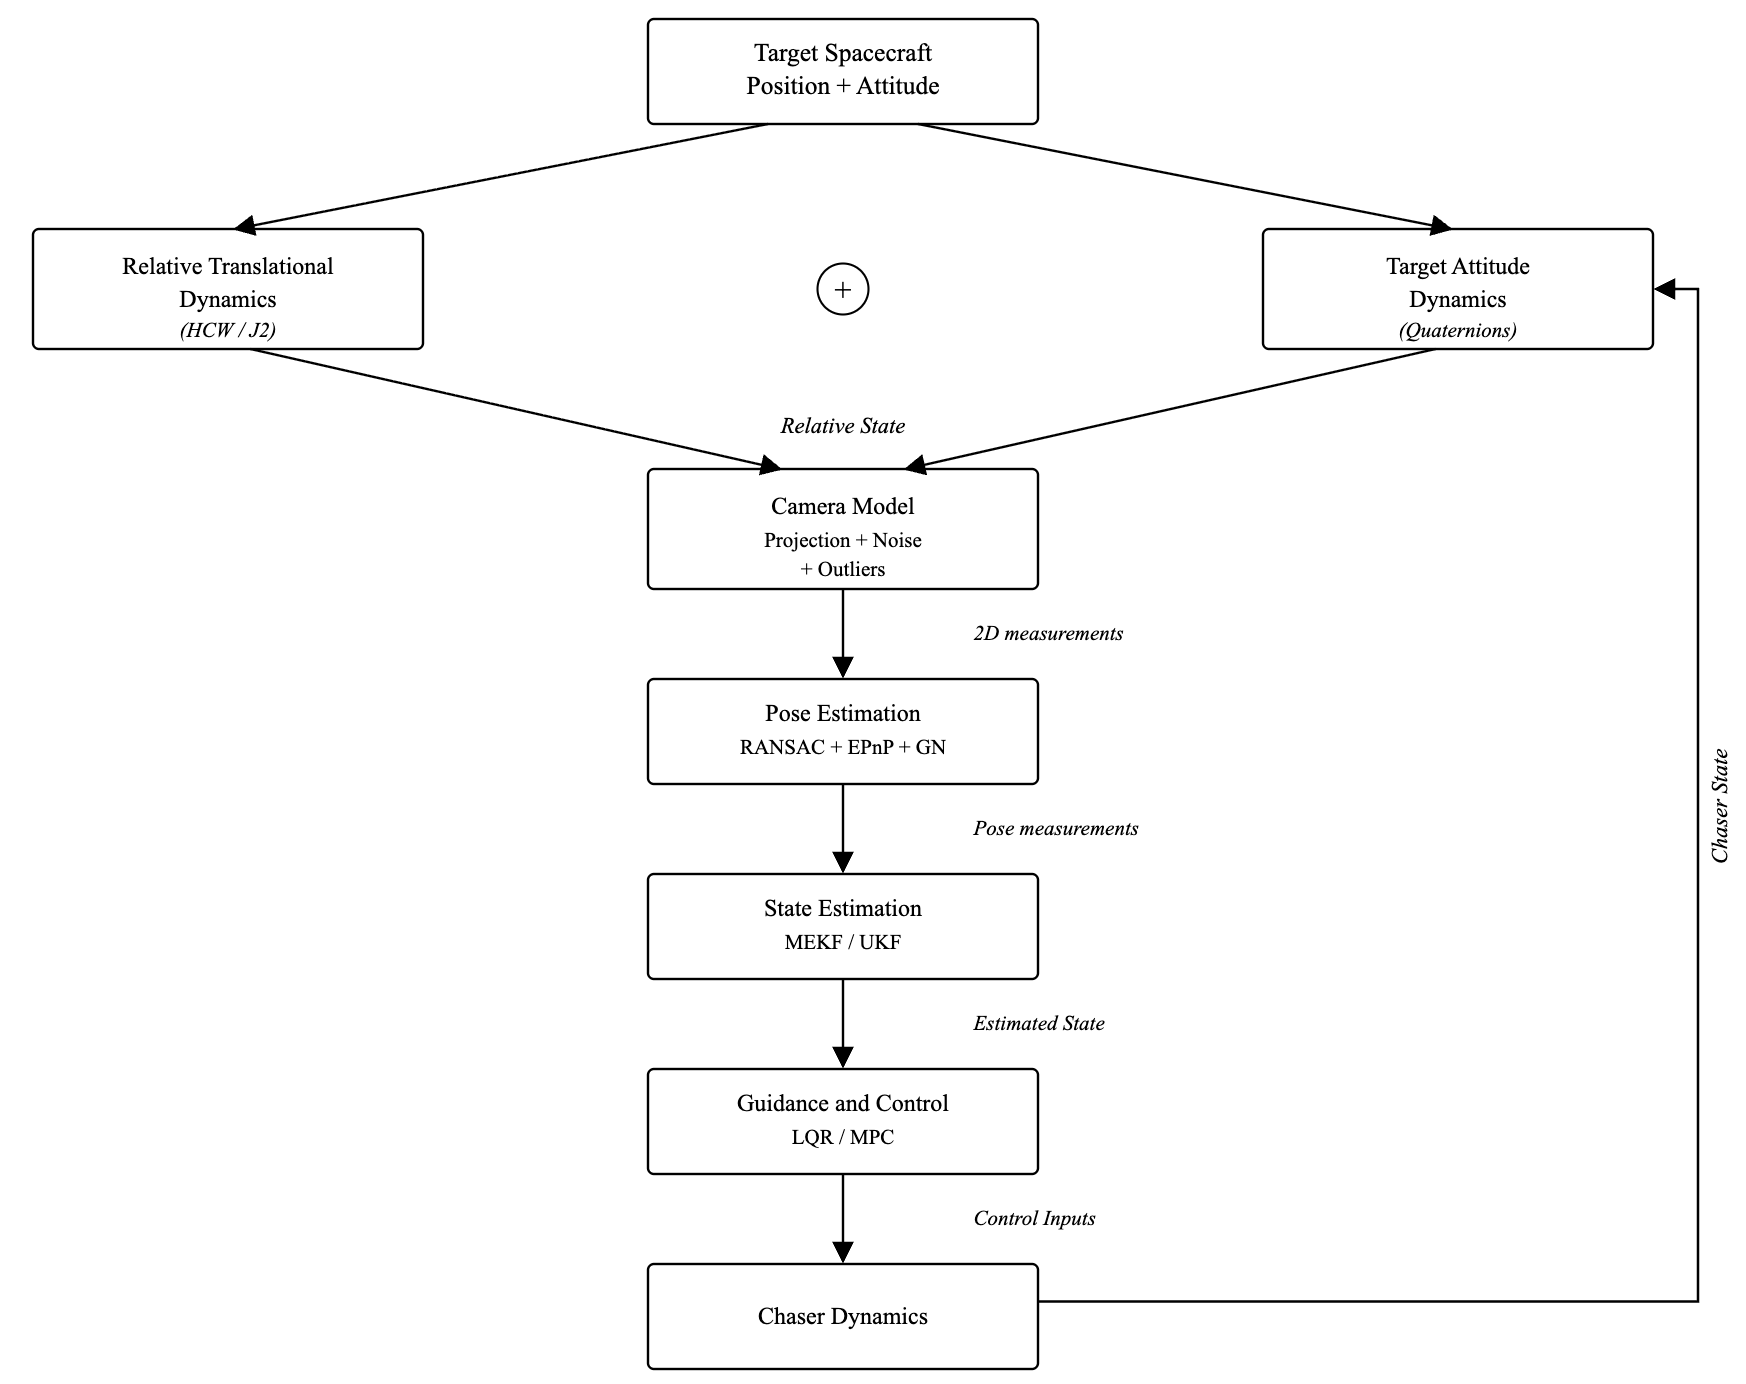
\includegraphics[width=\columnwidth]{figures/system_arch.png}
    \caption{Closed-loop architecture of the proposed vision-based
    autonomous spacecraft rendezvous framework.}
    \label{fig:system_architecture}
\end{figure}

\subsection{Reference Frames and Relative State}

Absolute quantities use the Earth Centred Inertial frame; the relative state
uses the target-centred Local Vertical Local Horizontal (LVLH) frame, with
radial axis $\hat{\mathbf{x}}$ from the Earth toward the target,
$\hat{\mathbf{z}}$ along the target orbital angular momentum and
$\hat{\mathbf{y}}=\hat{\mathbf{z}}\times\hat{\mathbf{x}}$. The translational
relative state is
$\mathbf{x}_{\mathrm{rel}}=[\mathbf{r}^{T}\ \mathbf{v}^{T}]^{T}$,
and the target attitude is carried as a unit quaternion $\mathbf{q}$ with
body-frame angular velocity $\boldsymbol{\omega}$, giving the attitude state
$\mathbf{x}_{\mathrm{att}}=[\mathbf{q}^{T}\ \boldsymbol{\omega}^{T}]^{T}$
subject to $\mathbf{q}^{T}\mathbf{q}=1$. The Hamilton convention is used
throughout; the dynamics and vision models store $\mathbf{q}$ scalar-first,
the estimator scalar-last as
$\mathbf{q}=[q_x\ q_y\ q_z\ q_w]^{T}$.

\subsection{Relative Orbital Dynamics}

For a near-circular reference orbit in LEO the relative translational
dynamics are the Hill--Clohessy--Wiltshire (HCW) equations
\cite{clohessy1960}. With mean motion $n=\sqrt{\mu/a^3}$, for gravitational
parameter $\mu$ and target semi-major axis $a$, the controlled equations are
\begin{equation}
\begin{aligned}
    \ddot{x} - 2n\dot{y} - 3n^2x &= f_x, \\
    \ddot{y} + 2n\dot{x} &= f_y, \\
    \ddot{z} + n^2z &= f_z,
\end{aligned}
\end{equation}
where $\mathbf{u}=[f_x\ f_y\ f_z]^{T}$ is the chaser control acceleration in
the LVLH frame. These assemble into the linear time-invariant form
$\dot{\mathbf{x}}_{\mathrm{rel}}
=\mathbf{A}_{\mathrm{HCW}}\mathbf{x}_{\mathrm{rel}}+\mathbf{B}\mathbf{u}$
with $\mathbf{B}=[\mathbf{0}_{3\times3}\ \ \mathbf{I}_{3}]^{T}$, whose
closed-form state transition is used by the guidance and control algorithms.
A higher-fidelity numerical path is retained for comparison, adding the
second-degree zonal harmonic $J_2$ to the two-body acceleration; it is not
exercised by any result reported here, where the unmodelled disturbance is
instead injected as a white acceleration on the true trajectory alone.

\subsection{Target Attitude Dynamics}

The target is a rigid body in potentially tumbling motion. Its quaternion
gives the direction cosine matrix $\mathbf{C}(\mathbf{q})$ from the target
body frame to the inertial frame, and the attitude evolves as
\begin{equation}
    \dot{\mathbf{q}}
    =
    \tfrac{1}{2}\mathbf{\Xi}(\mathbf{q})\boldsymbol{\omega},
    \qquad
    \mathbf{I}\dot{\boldsymbol{\omega}}
    =
    \boldsymbol{\tau}
    -\boldsymbol{\omega}\times(\mathbf{I}\boldsymbol{\omega}),
\end{equation}
with $\mathbf{\Xi}(\mathbf{q})$ the quaternion kinematic matrix, $\mathbf{I}$
the target inertia tensor and $\boldsymbol{\tau}$ the external body-frame
torque, zero in the scenarios considered here. Propagation uses an adaptive
high-order integrator with the quaternion renormalised each step. For
torque-free motion the rotational kinetic energy
$\tfrac{1}{2}\boldsymbol{\omega}^{T}\mathbf{I}\boldsymbol{\omega}$ and the
inertial angular momentum
$\mathbf{C}(\mathbf{q})\mathbf{I}\boldsymbol{\omega}$ are invariant, and are
monitored as numerical consistency checks.

\subsection{Camera Projection Model}

The perception module models a monocular camera on the chaser observing
fifteen analytically defined body-frame landmarks $\mathbf{P}_i^{b}$ on a
parametric Ariane 44L upper stage, distributed over the nose, mid-body ring
and nozzle, with the body-frame origin at the cylindrical centre and its
$x$-axis along the symmetry axis. The camera sits at the chaser with no
mounting rotation or lever arm, so the target attitude supplies the rotation
$\mathbf{R}_{bt}\in SO(3)$ and the HCW relative position $\mathbf{r}$ the
translation,
\begin{equation}
    \mathbf{P}_i^{c} = \mathbf{R}_{bt}\mathbf{P}_i^{b} + \mathbf{r}.
\end{equation}
Landmarks are mapped to the image by the pinhole model, which defines the
projection $\pi(\cdot)$,
\begin{equation}
    \mathbf{p}_i
    =
    \begin{bmatrix} u_i \\ v_i \end{bmatrix}
    =
    \begin{bmatrix}
        f_x X_i^c/Z_i^c + c_x \\ f_y Y_i^c/Z_i^c + c_y
    \end{bmatrix},
    \quad
    \tilde{\mathbf{p}}_i = \mathbf{p}_i + \boldsymbol{\eta}_i,
\end{equation}
for focal lengths $f_x,f_y$ and principal point $(c_x,c_y)$, with zero-mean
Gaussian pixel noise
$\boldsymbol{\eta}_i\sim\mathcal{N}(\mathbf{0},\sigma_{\mathrm{px}}^2\mathbf{I}_2)$
added independently to each landmark. The model supports the Brown--Conrady
radial and tangential distortion polynomial, disabled here with
$k_1=k_2=p_1=p_2=0$. A landmark is visible only when
$Z_i^c>0$ and $(u_i,v_i)$ falls inside the $W\times H$ image; the surviving
correspondences $\{\tilde{\mathbf{p}}_i \leftrightarrow
\mathbf{P}_i^b\}_{i=1}^{N}$ are the input to the pose-estimation stage.
Controlled correspondence outliers can also be injected to test that stage
under degraded observations. Camera and noise values are listed in
Table~\ref{tab:experimental_parameters}.

\subsection{Perspective-$n$-Point Pose Estimation}

Given $N$ correspondences, the pose-estimation stage recovers
$\mathbf{R}_{bt}\in SO(3)$ and $\mathbf{t}\in\mathbb{R}^{3}$ for which
$\mathbf{P}_i^c=\mathbf{R}_{bt}\mathbf{P}_i^b+\mathbf{t}$ reprojects
consistently onto the measured image points. The initial estimate uses the
Efficient Perspective-$n$-Point (EPnP) algorithm \cite{lepetit2009epnp},
which requires at least four correspondences, writes each landmark as an
affine combination of four virtual control points, and solves the resulting
homogeneous system $\mathbf{M}\mathbf{x}=\mathbf{0}$ through the null space
of $\mathbf{M}$ by singular value decomposition
(Section~\ref{sec:epnp_gn}). Among the candidate null-space solutions the one
with the lowest mean reprojection error satisfying the positive-depth
chirality constraint is selected, the landmark configuration reconstructed
from the barycentric coefficients, and the pose
$(\hat{\mathbf{R}}_{bt},\hat{\mathbf{t}})$ recovered by a rigid-body
absolute-orientation solution, whose quality is the reprojection error
\begin{equation}
    e_i^{\mathrm{rep}}
    =
    \left\|
    \tilde{\mathbf{p}}_i
    -
    \pi\left(\hat{\mathbf{R}}_{bt}\mathbf{P}_i^b+\hat{\mathbf{t}}\right)
    \right\|_2,
    \qquad
    \bar e_{\mathrm{rep}}
    =
    \frac{1}{N}\sum_{i=1}^{N} e_i^{\mathrm{rep}} .
\end{equation}
An optional nonlinear refinement of this cost is applied on top of the EPnP
solution; because a global rotation-vector parameterisation is singular at
$\theta=\pi$, it is formulated on the $SO(3)$ manifold
(Section~\ref{sec:pnp_manifold}) and is not used in the closed-loop pipeline.

\subsubsection{RANSAC-Based Outlier Rejection}

To tolerate incorrect correspondences the EPnP solver is wrapped in a RANSAC
stage \cite{fischler1981ransac} following the locally optimised strategy of
Chum and Matas~\cite{chum2003loransac}: a minimal subset is sampled, an EPnP
hypothesis generated, and correspondences with
$e_i^{\mathrm{rep}}<\tau_{\mathrm{rep}}$ counted as inliers. The largest
consensus set wins, with mean inlier reprojection error as the tie-break, and
the pose is refitted on its inliers. Sampling terminates adaptively once
\begin{equation}
    k \;\geq\; \frac{\log(1-p)}{\log\!\left(1-w^{s}\right)},
\end{equation}
where $w$ is the observed inlier ratio, $s$ the minimal sample size and $p$
the desired confidence level, subject to the iteration budget and inlier
threshold of Table~\ref{tab:experimental_parameters}.

\subsection{State Estimation}

Pose solutions are instantaneous and corrupted by image noise and pose-solver
error, so a recursive estimator supplies a temporally consistent relative
state. A Multiplicative Extended Kalman Filter (MEKF) \cite{markley2003} and
an error-state Unscented Kalman Filter (UKF) \cite{julier2004} are compared,
sharing nominal state, process and measurement models so that the filtering
formulation is the only difference. The nominal navigation state is
\begin{equation}
    \mathbf{x}
    =
    \begin{bmatrix}
        \mathbf{r}^{T} & \mathbf{v}^{T} &
        \mathbf{q}^{T} & \boldsymbol{\omega}^{T}
    \end{bmatrix}^{T},
    \quad
    \delta\mathbf{x}
    =
    \begin{bmatrix}
        \delta\mathbf{r}^{T} & \delta\mathbf{v}^{T} &
        \delta\boldsymbol{\alpha}^{T} & \delta\boldsymbol{\omega}^{T}
    \end{bmatrix}^{T},
\end{equation}
with $\|\mathbf{q}\|=1$. Because additive quaternion perturbations violate
that constraint, the covariance is carried in the 12-dimensional error state,
$\delta\boldsymbol{\alpha}$ being the small-angle attitude error. The nominal
state is propagated through the nonlinear dynamics and the covariance through
the error-state transition matrix $\mathbf{F}_k$,
\begin{equation}
    \mathbf{x}_{k+1}^{-} = f(\mathbf{x}_{k}^{+},\Delta t),
    \qquad
    \mathbf{P}_{k+1}^{-}
    =
    \mathbf{F}_{k}\mathbf{P}_{k}^{+}\mathbf{F}_{k}^{T}+\mathbf{Q}_{k},
\end{equation}
where $\Delta t$ is the sampling interval and $\mathbf{Q}_k$ is
acceleration-driven as derived in Section~\ref{sec:process_noise}.

The measurement supplied to the estimator is a relative translation and a
target attitude. In the filter-isolation experiment it is generated directly
from the true state with additive Gaussian noise,
\begin{equation}
    \mathbf{z}_{k}
    =
    \begin{bmatrix}
        \mathbf{r}_{k}^{\mathrm{true}}\\
        \boldsymbol{\rho}_{k}^{\mathrm{true}}
    \end{bmatrix}
    +
    \begin{bmatrix}
        \boldsymbol{\nu}_{r,k}\\ \boldsymbol{\nu}_{\rho,k}
    \end{bmatrix},
    \qquad
    \mathbf{R}
    =
    \begin{bmatrix}
        \sigma_{\mathrm{pos}}^{2}\mathbf{I}_{3} & \mathbf{0}\\
        \mathbf{0} & \sigma_{\mathrm{att}}^{2}\mathbf{I}_{3}
    \end{bmatrix},
\end{equation}
where $\boldsymbol{\rho}$ is the rotation vector of the target attitude and
the noise standard deviations are those of
Table~\ref{tab:experimental_parameters}. The complete vision-to-estimation
pipeline is evaluated separately in Section~\ref{sec:results}.

\subsubsection{Multiplicative Extended Kalman Filter}

With predicted measurement $\hat{\mathbf{z}}_{k}=h(\mathbf{x}_{k}^{-})$,
innovation $\mathbf{y}_{k}=\mathbf{z}_{k}-\hat{\mathbf{z}}_{k}$ and
innovation covariance $\mathbf{S}_{k}=\mathbf{H}_{k}\mathbf{P}_{k}^{-}
\mathbf{H}_{k}^{T}+\mathbf{R}_{k}$, the gain and error-state correction are
$\mathbf{K}_{k}=\mathbf{P}_{k}^{-}\mathbf{H}_{k}^{T}\mathbf{S}_{k}^{-1}$ and
$\delta\mathbf{x}_{k}=\mathbf{K}_{k}\mathbf{y}_{k}$, the attitude component of $\mathbf{y}_k$ being formed multiplicatively on
$SO(3)$, which makes $\mathbf{H}_k$ exact and constant
(Section~\ref{sec:mekf_residual}). Translational and angular-velocity
corrections are applied additively, while the attitude correction is applied
multiplicatively to the nominal attitude,
\begin{equation}
    \mathbf{q}_{k}^{+}
    =
    \operatorname{norm}
    \left(
        \operatorname{Exp}(\delta\boldsymbol{\alpha}_{k})
        \otimes
        \mathbf{q}_{k}^{-}
    \right),
\end{equation}
and the covariance is updated in Joseph form,
\begin{equation}
    \mathbf{P}_{k}^{+}
    =
    (\mathbf{I}-\mathbf{K}_{k}\mathbf{H}_{k})
    \mathbf{P}_{k}^{-}
    (\mathbf{I}-\mathbf{K}_{k}\mathbf{H}_{k})^{T}
    +
    \mathbf{K}_{k}\mathbf{R}_{k}\mathbf{K}_{k}^{T},
\end{equation}
symmetrised after prediction and update. Measurements statistically
inconsistent with the prediction are rejected by a Mahalanobis gate on the
squared normalised innovation,
$d_k^2=\mathbf{y}_{k}^{T}\mathbf{S}_{k}^{-1}\mathbf{y}_{k}\leq\gamma$, with
$\gamma$ the chi-square threshold of
Table~\ref{tab:experimental_parameters}; a failing measurement is discarded
and the predicted state retained. The attitude part of the innovation is
expressed as a principal rotation vector before the distance is evaluated.

\subsubsection{Unscented Kalman Filter}

The UKF replaces the analytic linearisation by propagating sigma points
through the nonlinear models, using the same 12-dimensional error state. For
$n_x=12$ the scaled unscented transform sets
\begin{equation}
    \lambda = \alpha^2(n_x+\kappa)-n_x,
    \qquad
    W_0^{(m)} = \frac{\lambda}{n_x+\lambda},
\end{equation}
so that both the sigma-point spread and the centre weight are controlled by
$\alpha$; the sigma points and the remaining weights
follow the standard scaled transform \cite{julier2004}. Each error-state sigma
point is applied to the nominal state --- attitude perturbations
multiplicatively, preserving the unit-norm constraint --- and propagated
through the relative translational and attitude dynamics, giving the
cross-covariance $\mathbf{P}_{xz}$ and the innovation covariance
$\mathbf{P}_{zz}$, from which
$\mathbf{K}=\mathbf{P}_{xz}\mathbf{P}_{zz}^{-1}$ and
$\delta\mathbf{x}=\mathbf{K}(\mathbf{z}-\hat{\mathbf{z}})$, the attitude
correction again applied multiplicatively. The implemented filter uses
$\alpha=0.5$, $\beta=2$ and $\kappa=0$.

\subsection{Guidance and Control}

The guidance-and-control module drives the chaser with either a Linear
Quadratic Regulator (LQR) or a receding-horizon Model Predictive Controller
(MPC), both acting on the HCW relative dynamics. The MPC imposes an explicit
thrust constraint and, during the terminal phase, an approach-cone constraint
formulated as a softened second-order cone (Section~\ref{sec:cone}). The
commanded acceleration $\mathbf{u}$ updates the chaser state and produces the
next camera observation, closing the perception--navigation--control loop.

\subsection{Refinement of the EPnP Control-Point Coefficients}
\label{sec:epnp_gn}

Writing the $N$ world points as affine combinations of control points,
$\mathbf{P}_i = \sum_{j} \alpha_{ij}\,\mathbf{c}_j$ with
$\sum_j \alpha_{ij} = 1$, the projection equations stack into
$\mathbf{M}\mathbf{x} = \mathbf{0}$, where $\mathbf{x}$ collects the control
points in the camera frame. The solution lies in the null space of
$\mathbf{M}$,
\begin{equation}
\mathbf{x} = \sum_{k=1}^{n} \beta_k \mathbf{v}_k ,
\label{eq:epnp_null}
\end{equation}
and the coefficients $\beta_k$ are fixed by requiring that the
inter-control-point distances be preserved:
\begin{equation}
\bigl\| \textstyle\sum_k \beta_k (\mathbf{v}_k^{[i]} - \mathbf{v}_k^{[j]}) \bigr\|^2
= \| \mathbf{c}_i - \mathbf{c}_j \|^2 ,
\qquad i < j .
\label{eq:epnp_dist}
\end{equation}

Equation~\eqref{eq:epnp_dist} is quadratic in $\boldsymbol{\beta}$.
Linearising in the products $b_{kl} = \beta_k \beta_l$ gives a linear system
$\mathbf{L}\mathbf{b} = \boldsymbol{\rho}$ whose least-squares solution yields
an initial $\boldsymbol{\beta}$ by relinearisation,
$\beta_1 = \sqrt{|b_{11}|}$ and $\beta_k = b_{1k}/\beta_1$. This is an
\emph{initialisation}, not the answer, and treating it as the answer costs
roughly a factor of four in accuracy (Sec.~\ref{sec:res_pose}). We refine
$\boldsymbol{\beta}$ by Gauss--Newton directly on \eqref{eq:epnp_dist}. With
$\mathbf{D}_{ij}$ the matrix whose $k$-th column is
$\mathbf{v}_k^{[i]} - \mathbf{v}_k^{[j]}$ and
$\mathbf{d}_{ij} = \mathbf{D}_{ij}\boldsymbol{\beta}$, the residual and its
Jacobian are
\begin{align}
f_{ij}(\boldsymbol{\beta}) &= \mathbf{d}_{ij}^{\top}\mathbf{d}_{ij}
                              - \|\mathbf{c}_i - \mathbf{c}_j\|^2 ,
\label{eq:epnp_resid}\\
\frac{\partial f_{ij}}{\partial \beta_m}
  &= 2\, \mathbf{d}_{ij}^{\top} \mathbf{D}_{ij}\,\mathbf{e}_m .
\label{eq:epnp_jac}
\end{align}
Ten iterations of $\boldsymbol{\beta} \leftarrow \boldsymbol{\beta} +
\boldsymbol{\delta}$, with $\boldsymbol{\delta}$ the least-squares solution of
$\mathbf{J}\boldsymbol{\delta} = -\mathbf{f}$, suffice in every case tested.

\paragraph{The coplanar case.}
The control points are the centroid plus the principal axes of the point
cloud, scaled by the corresponding singular values. When the cloud is
coplanar the third singular value vanishes, so a fourth control point
coincides with the centroid, the barycentric system becomes singular, and
three columns of $\mathbf{M}$ vanish identically --- giving $\mathbf{M}$ a
four-dimensional null space for algebraic rather than geometric reasons. The
planar configuration must therefore be detected, from $s_3 / s_1 < \epsilon$,
and parameterised with \emph{three} control points, so that
$\mathbf{x} \in \mathbb{R}^{9}$ and $\mathbf{M}$ is $2N \times 9$.
Approximately 3\% of random six-point subsets of the target's keypoint set
are exactly coplanar, so this is not an edge case.

\subsection{Pose Refinement on the $SO(3)$ Manifold}
\label{sec:pnp_manifold}

The refinement stage minimises the reprojection cost
\begin{equation}
E(\mathbf{R}, \mathbf{t}) = \sum_{i} w_i \,
\bigl\| \tilde{\mathbf{p}}_i - \pi(\mathbf{R}\mathbf{P}_i + \mathbf{t}) \bigr\|^2 .
\label{eq:lm_cost}
\end{equation}
Parameterising $\mathbf{R} = \exp([\mathbf{r}]_\times)$ by a \emph{global}
rotation vector is convenient but singular at $\|\mathbf{r}\| = \pi$, where the
derivative of the exponential map is unbounded --- not a remote possibility
here, since a camera whose boresight is aligned with a world axis produces
$\operatorname{tr}(\mathbf{R}) = -1$ exactly, i.e.\ $\theta = \pi$, and such
poses are the natural fixtures for an on-axis approach. We therefore carry
$\mathbf{R}$ as a matrix and optimise over a local increment. Using a
left-multiplicative update,
\begin{equation}
\mathbf{R} \leftarrow \exp([\boldsymbol{\delta\omega}]_\times)\,\mathbf{R},
\qquad
\mathbf{t} \leftarrow \mathbf{t} + \boldsymbol{\delta t} ,
\label{eq:lm_update}
\end{equation}
and noting that $\exp([\boldsymbol{\delta}]_\times)\mathbf{v} \approx
\mathbf{v} - [\mathbf{v}]_\times \boldsymbol{\delta}$, the Jacobian blocks at
$\boldsymbol{\delta} = \mathbf{0}$ are
\begin{equation}
\frac{\partial \mathbf{P}^c_i}{\partial \boldsymbol{\delta\omega}}
  = -[\mathbf{R}\mathbf{P}_i]_\times ,
\qquad
\frac{\partial \mathbf{P}^c_i}{\partial \boldsymbol{\delta t}} = \mathbf{I}_3 ,
\label{eq:lm_jac}
\end{equation}
so that with the perspective Jacobian
\begin{equation}
\frac{\partial \pi}{\partial \mathbf{P}^c}
= \begin{bmatrix}
f_x / Z & 0 & -f_x X / Z^2 \\
0 & f_y / Z & -f_y Y / Z^2
\end{bmatrix}
\label{eq:proj_jac}
\end{equation}
the stacked Jacobian is
$\mathbf{J}_i = (\partial \pi / \partial \mathbf{P}^c)\,
[-[\mathbf{R}\mathbf{P}_i]_\times \;\; \mathbf{I}_3]$.
Because $\boldsymbol{\delta\omega}$ is always near zero, the local
parameterisation is well conditioned wherever the optimiser is, and the
singularity cannot be reached. Two further conditions keep the iteration
honest. The residual and the Jacobian must be evaluated at the same point ---
clamping $Z$ in one and not the other lets Levenberg--Marquardt accept steps
that lower a cost it is not actually computing, and the translation then
diverges without bound while the reported cost stays finite. And chirality
must be enforced: any pose placing a weighted point at or behind the camera
plane is assigned infinite cost and rejected, so failure is visible rather
than silent.

\subsection{Multiplicative Attitude Residual}
\label{sec:mekf_residual}

Position enters the residual as a difference in the usual way; attitude
cannot, and the reason is worth setting out because the naive form is
superficially reasonable. With $\hat{\mathbf{q}}$ the filter's estimate,
encoding both attitudes as global rotation vectors and subtracting,
$\boldsymbol{\nu}_{att} = \log(\mathbf{q}_{meas}) - \log(\hat{\mathbf{q}})$,
fails at $\theta = \pi$: two attitudes separated by an arbitrarily small
rotation, one either side of $\pi$, map to nearly antipodal rotation vectors,
so a vanishing attitude error produces a residual of magnitude $2\pi$. The
linearised residual is then meaningless, and the Jacobian condition number
grows without bound as $\theta \to \pi$. The residual must instead be formed
on the group and expressed in the tangent space at the estimate,
\begin{equation}
\boldsymbol{\delta\alpha}
  = \log\!\bigl( \mathbf{q}_{meas} \otimes \hat{\mathbf{q}}^{-1} \bigr) ,
\label{eq:att_residual}
\end{equation}
where $\log(\cdot)$ returns the rotation vector of its argument and the sign of
the relative quaternion is chosen so that its scalar part is non-negative,
selecting the short rotation. This is exact for every attitude, and it has a
second benefit. Because the error state is defined by the same
left-multiplicative perturbation,
$\mathbf{q} = \exp(\tfrac{1}{2}\boldsymbol{\delta\alpha}) \otimes
\hat{\mathbf{q}}$, the residual \emph{is} the attitude error state to first
order, and the measurement Jacobian becomes exact and constant:
\begin{equation}
\mathbf{H} =
\begin{bmatrix}
\mathbf{I}_3 & \mathbf{0} & \mathbf{0} & \mathbf{0} \\
\mathbf{0} & \mathbf{0} & \mathbf{I}_3 & \mathbf{0}
\end{bmatrix} .
\label{eq:H_exact}
\end{equation}
No finite differencing is required, and $\mathbf{R}_{att} = \sigma_{att}^2
\mathbf{I}_3$ becomes a genuine tangent-space covariance rather than an
approximation. The measurement noise must be injected on the same side for
this to hold: a physical attitude perturbation is
$\mathbf{q}_{meas} = \exp(\tfrac{1}{2}\boldsymbol{\eta}) \otimes \mathbf{q}$
with $\boldsymbol{\eta} \sim \mathcal{N}(\mathbf{0},
\sigma_{att}^2\mathbf{I}_3)$.

\subsection{Acceleration-Driven Process Noise}
\label{sec:process_noise}

The dominant unmodelled effects on the relative translation --- differential
$J_2$, differential drag, thruster execution error --- act as an
\emph{acceleration}, so the process noise must drive position and velocity
jointly. Treating the disturbance as white acceleration of density
$\sigma_a$ over a step $\Delta t$ gives the standard kinematic block
\begin{equation}
\begin{bmatrix}
\mathbf{Q}_{rr} & \mathbf{Q}_{rv} \\
\mathbf{Q}_{vr} & \mathbf{Q}_{vv}
\end{bmatrix}
= \sigma_a^2
\begin{bmatrix}
\tfrac{1}{3}\Delta t^3 \mathbf{I}_3 & \tfrac{1}{2}\Delta t^2 \mathbf{I}_3 \\
\tfrac{1}{2}\Delta t^2 \mathbf{I}_3 & \Delta t\, \mathbf{I}_3
\end{bmatrix},
\label{eq:Q_kin}
\end{equation}
with the same structure on the attitude and rate block for an angular
acceleration density. The off-diagonal terms are not optional: position and
velocity errors driven by a common acceleration are correlated, and a diagonal
$\mathbf{Q}$ asserts that they are not, which weakens the information a
position measurement carries about velocity. A diagonal alternative that
models position as an independent random walk is worse still --- a position
noise of $0.05$~m per step contributes
$\mathbf{Q}_{rr} = 2.5 \times 10^{-3}$~m$^2$, roughly three hundred times the
$8.3 \times 10^{-6}$~m$^2$ that a physically plausible
$5 \times 10^{-4}$~m/s$^2$ disturbance produces over a one-second step. The
filter is then needlessly conservative, and its $\mathbf{Q}$ describes a
disturbance that is not present in the truth, so the consistency statistics of
Eq.~\eqref{eq:nis} become uninformative.

\subsection{Approach Corridor as a Second-Order Cone}
\label{sec:cone}

The terminal approach is confined to a cone of half-angle $\theta_c$ about the
$+x$ (radial) approach axis. For a predicted position
$\mathbf{r}_k = [x_k,\ y_k,\ z_k]^{\top}$ the constraint is
\begin{equation}
\sqrt{y_k^2 + z_k^2} \;\le\; x_k \tan\theta_c ,
\qquad k = 0,\dots,N-1 .
\label{eq:cone}
\end{equation}
Three properties of \eqref{eq:cone} matter and are each easy to lose. It is a
\emph{cone}, not a wedge: both transverse components appear, and constraining
$|y_k|$ alone leaves the cross-track axis free. It is \emph{signed}: the
right-hand side must be non-negative, so \eqref{eq:cone} implies
$x_k \ge 0$, whereas replacing $x_k$ by $|x_k|$ mirrors the corridor into
$x < 0$ and is satisfied by a chaser sitting behind the target. And the
constrained quantity is the predicted state
$\mathbf{X}(\mathbf{U}) = \mathbf{S}_x \mathbf{e} + \mathbf{S}_u \mathbf{U}$;
evaluating the radius on the free response $\mathbf{S}_x\mathbf{e}$ makes the
right-hand side independent of the decision variable, and the constraint
ceases to constrain anything. Written for a nonlinear-programming solver,
\eqref{eq:cone} becomes
$g_k(\mathbf{U}) \ge 0$ with
\begin{equation}
g_k(\mathbf{U}) = \tan\theta_c \; x_k(\mathbf{U})
   - \sqrt{y_k(\mathbf{U})^2 + z_k(\mathbf{U})^2 + \varepsilon^2},
\label{eq:cone_g}
\end{equation}
where $\varepsilon$ (here $10^{-6}$~m) keeps $g_k$ differentiable on the axis
at the cost of a marginally conservative constraint. The gradient is
\begin{equation}
\nabla_{\mathbf{U}} g_k = \tan\theta_c \, \mathbf{S}_u^{x,k}
 - \frac{y_k \mathbf{S}_u^{y,k} + z_k \mathbf{S}_u^{z,k}}
        {\sqrt{y_k^2 + z_k^2 + \varepsilon^2}} ,
\label{eq:cone_grad}
\end{equation}
with $\mathbf{S}_u^{x,k}$ the row of $\mathbf{S}_u$ selecting $x_k$.

Imposed as a hard constraint, \eqref{eq:cone} destroys recursive feasibility:
once the chaser lies outside the cone there may be no admissible input
returning the first predicted state to it, and the quadratic program is
infeasible. Since an infeasible solve is what produces a silent zero-thrust
command, we soften the corridor with slack $s_k \ge 0$ under a linear penalty,
\begin{equation}
\min_{\mathbf{U},\,\mathbf{s}} \;
\tfrac{1}{2}\mathbf{U}^{\top}\mathbf{H}\mathbf{U} + \mathbf{f}^{\top}\mathbf{U}
+ \rho \sum_{k} s_k
\quad \text{s.t.} \quad g_k(\mathbf{U}) + s_k \ge 0 ,
\label{eq:cone_soft}
\end{equation}
which is always feasible and drives $s_k \to 0$ whenever the hard constraint
can be met. The corridor solve is judged on the quantity it exists to reduce,
$\sum_k \max(0, -g_k)$, rather than on the solver's own convergence flag, and
is attempted only when the box-constrained optimum already violates
\eqref{eq:cone} --- an active-set shortcut that leaves the solution unchanged
when the corridor is inactive and reduces the per-step cost by two orders of
magnitude.


\section{Experimental Methodology}

We investigate the proposed vision-based rendezvous architecture with a set of controlled numerical experiments. Each main element is independently tested before investigating the full navigation-and-control pipeline. We move from analytically validating the dynamics through to estimating the visual poses, robust estimation, recursive state estimation, guidance-and-control, and lastly end-to-end Monte Carlo testing. 

This allows us to examine any numerical and algorithmic errors separate from the effects at the system level. 

Specifically, we demonstrate validity of the dynamics model against a known analytic solution and then characterising the pose-estimation pipeline’s sensitivity to image noise and outliers. We then examine the state estimators using a controlled measurement model and the fullvision--estimation--control pipeline using simulate camera measurements. All experiments use the same parameters of the target-spacecraft and the camera model introduced in sectionIII unless stated otherwise. A random seed will be chosen that will remain constant within a single Monte Carlo trial to allow for reproduceability.

\subsection{Experimental Objectives}

The experiment campaign is structured around six main investigations.

\begin{enumerate}

\item \textbf{Dynamics validation:} The numerical implementation of relative dynamics is verified against the analytical HCW state transition solution, and numerical solver convergence is analyzed.

\item \textbf{Pixel-noise sensitivity:} The image plane measurement noise level is varied and its impact on EPnP pose is analyzed along with the effectiveness of the nonlinear pose refinement stage.

\item \textbf{Outlier robustness:} RANSAC relative pose is analyzed under an increasing amount of outliers.

\item \textbf{State-estimation comparison:} Under an assumed Gaussian measurement model, the MEKF and UKF stat estimation algorithms are compared.

\item \textbf{Guidance and control comparison:} Relative rendezvous under HCW dynamics is assessed for guidance and control, using a receding-horizon MPC as well as a LQR controller.

\item \textbf{End-to-end robustness:} The overall vision to control architecture performance is assessed for various values of pixel noise based on Monte Carlo simulations.

\end{enumerate}

Consequently the experiments can be structured to address three escalating and broader issues : that the constituent mathematical models hold , that individual navigation and control algorithms perform in presence of unwanted perturbations , and finally that the overall architecture continues to function correctly when individual components interact with each other.

\subsection{Simulation Environment and Common Parameters}

All simulation work is conducted on a numerical simulation infrastructure developed in Python. Relative translational dynamics are modeled in the LVLH reference frame with the HCW equations while target motion in attitude is propagated by a built-in rigid body attitude dynamics model. Numerical propagation is performed with standard fourth-order Runge-Kutta integration in modules that require it.

A parametric Ariane 44L upper stage geometry serves as the target spacecraft, containing 15 analytical keypoints in its body frame coordinates; which are then projected to the imaging sensors with the use of a calibrated camera model given in Section III-D.

Experiments with full images use $1024 \times 1024$ pixel frames with noise added to the ideal projected keypoints through a zero-mean Gaussian. Unless otherwise stated standard pixel noise level of $\sigma_{\mathrm{px}}=1.5$ px is utilized for all standard vision experiments.

Table~\ref{tab:experimental_parameters} summarises the standard simulation parameters used throughout the experimental campaign.
\begin{table}[t]
\centering
\caption{Common simulation and experimental parameters.}
\label{tab:experimental_parameters}
\begin{tabular}{lc}
\toprule
\textbf{Parameter} & \textbf{Value} \\
\midrule
Camera image size & $1024\times1024$ px \\
Target keypoints & 15 \\
Nominal pixel noise & $1.5$ px \\
HCW initial range (Exp. D) & 50 m \\
Filter sampling interval & 10 s \\
Filter horizon (Exp. D) & 3000 s \\
MEKF/UKF position noise & 0.5 m \\
MEKF/UKF attitude noise & 0.05 rad \\
LQR/MPC control interval & 10 s \\
MPC prediction horizon & 20 steps \\
Maximum control input (Exp. E) & 0.1 m/s$^2$ \\
Maximum control input (Exp. F) & 0.3 m/s$^2$ \\
\bottomrule
\end{tabular}
\end{table}

\subsection{Dynamics Validation}

The relative translational dynamics are first validated independently of
the vision and estimation subsystems. Experiment A compares the
closed-form HCW state-transition formulation against numerical
integration using the DOP853 solver.

A periodic HCW trajectory with an initial radial amplitude of 100 m is
propagated for three orbital periods. The analytical state is evaluated
at the same time points as the numerical solution, and the position and
velocity discrepancies are computed as

\begin{equation}
    e_r(t)
    =
    \left\|
        \mathbf{r}_{\mathrm{analytical}}(t)
        -
        \mathbf{r}_{\mathrm{numerical}}(t)
    \right\|_2,
\end{equation}

and

\begin{equation}
    e_v(t)
    =
    \left\|
        \mathbf{v}_{\mathrm{analytical}}(t)
        -
        \mathbf{v}_{\mathrm{numerical}}(t)
    \right\|_2.
\end{equation}

The maximum errors over the complete propagation interval are used as
the primary validation metrics.

The numerical integration is initially performed using
$\mathrm{rtol}=10^{-12}$ and $\mathrm{atol}=10^{-14}$. A second
convergence experiment varies the relative tolerance over

\begin{equation}
    \mathrm{rtol}
    \in
    \left\{
    10^{-6},10^{-8},10^{-10},10^{-12},10^{-13}
    \right\},
\end{equation}

with $\mathrm{atol}=10^{-2}\mathrm{rtol}$. The resulting maximum
position and velocity discrepancies are used to verify convergence of
the numerical propagation.

\subsection{Pixel-Noise Sensitivity of Pose Estimation}

Experiment B evaluates the sensitivity of the visual pose-estimation
pipeline to image-plane measurement noise. The ideal two-dimensional
keypoint observations are corrupted using independent zero-mean
Gaussian noise,

\begin{equation}
    \tilde{\mathbf{u}}_i
    =
    \mathbf{u}_i
    +
    \boldsymbol{\eta}_i,
    \qquad
    \boldsymbol{\eta}_i
    \sim
    \mathcal{N}
    \left(
        \mathbf{0},
        \sigma_{\mathrm{px}}^2\mathbf{I}_2
    \right).
\end{equation}

The experiment considers

\begin{equation}
\sigma_{\mathrm{px}}
\in
\{0.1,\;0.25,\;0.5,\;1,\;1.5,\;2,\;3,\;5\}\ {\rm px}.
\end{equation}

For each noise level, 200 independent Monte Carlo trials are performed.
The raw EPnP solution is compared with the solution obtained after
nonlinear Gauss--Newton pose refinement.

The translation error is evaluated using the Euclidean norm,

\begin{equation}
    e_t =
    \left\|
        \hat{\mathbf{t}}-\mathbf{t}_{\mathrm{gt}}
    \right\|_2,
\end{equation}

while the rotational error is evaluated using the geodesic angle

\begin{equation}
    e_R
    =
    \cos^{-1}
    \left[
    \frac{
    \operatorname{tr}
    \left(
    \hat{\mathbf{R}}
    \mathbf{R}_{\mathrm{gt}}^{T}
    \right)-1
    }{2}
    \right].
\end{equation}

The mean reprojection error is additionally recorded to quantify the
image-space consistency of each recovered pose. Translation RMSE,
rotation error, and reprojection error are reported as functions of
pixel noise.

\subsection{Robustness to Image Outliers}

Experiment C evaluates the robustness of pose estimation to incorrect
keypoint correspondences. Inlier observations are corrupted with
Gaussian pixel noise of $\sigma_{\mathrm{px}}=1$ px. A controlled
fraction of the keypoints is then replaced with randomly generated
image coordinates distributed over the complete camera image.

The tested outlier fractions are

\begin{equation}
    f_{\mathrm{out}}
    \in
    \{0,\;5,\;10,\;20,\;30\}\%.
\end{equation}

For each condition, 200 independent trials are performed. Bare EPnP is
compared with the proposed RANSAC--EPnP configuration using a
2-pixel inlier threshold and a maximum of 500 RANSAC iterations.

A trial is classified as a failure if either the pose solver reports an
invalid solution or the recovered rotation error exceeds $15^\circ$.
The resulting failure rate is

\begin{equation}
    P_{\mathrm{fail}}
    =
    \frac{N_{\mathrm{invalid}}
    +
    N_{e_R>15^\circ}}
    {N_{\mathrm{trials}}}
    \times 100\%.
\end{equation}

Translation and rotation RMSE are computed over successful trials,
while the failure rate is computed over all trials. This distinction
prevents unsuccessful trials from being silently removed from the
robustness analysis.

\subsection{State-Estimation Evaluation}

Experiment D evaluates the recursive state-estimation stage by
comparing the MEKF and UKF under an identical controlled measurement
model. The purpose of this experiment is to isolate filter behavior
from the stochastic characteristics of the camera and PnP pipeline.

The simulated rendezvous begins at a 50-m along-track separation with
zero initial relative velocity. The target is assigned a slow
uncontrolled angular velocity of

\begin{equation}
    \boldsymbol{\omega}
    =
    [0.01,\;0.02,\;-0.015]^{T}\ {\rm rad/s}.
\end{equation}

The filter sampling interval is 10 s and the simulation contains 300
steps, corresponding to 3000 s.

The initial filter state contains deliberate errors of approximately
4 m in position and $17^\circ$ in attitude to represent a cold-start
condition. Both filters receive the same noisy pose measurement with

\begin{equation}
    \sigma_{\mathrm{pos}}=0.5~{\rm m},
    \qquad
    \sigma_{\mathrm{att}}=0.05~{\rm rad}.
\end{equation}

Position, attitude, and velocity errors are recorded throughout the
simulation. The root-mean-square error is computed as

\begin{equation}
    \mathrm{RMSE}
    =
    \sqrt{
    \frac{1}{N}
    \sum_{k=1}^{N}
    e_k^2
    }.
\end{equation}

Maximum position and attitude errors, the number of accepted
measurements, and wall-clock execution time are also recorded.

Importantly, this experiment uses direct synthetic Gaussian pose
measurements rather than pixel measurements generated by the camera
and PnP stages. Thus, the results characterize the filter comparison
under a controlled measurement distribution and should not be
interpreted as an end-to-end camera-navigation comparison.

\subsection{Guidance and Control Evaluation}

Experiment E compares an infinite-horizon discrete LQR controller with
a receding-horizon MPC controller for translational rendezvous under
HCW dynamics.

Both controllers start from the same relative state,

\begin{equation}
    \mathbf{x}_0
    =
    [0,\;50,\;0,\;0,\;0,\;0]^T,
\end{equation}

corresponding to a 50-m along-track separation and zero initial
relative velocity. The control interval is 10 s and the simulation
contains 200 control steps.

The LQR controller is obtained from the discrete algebraic Riccati
equation \cite{anderson1990}, while MPC \cite{mayne2000} uses a
20-step prediction horizon and the LQR solution as its terminal cost,
following the approach of Breger and How~\cite{breger2008} for
spacecraft proximity operations. Both controllers use identical state
and control weighting and a maximum control input magnitude of
$0.1~\mathrm{m/s^2}$.

The controllers are compared using final range,

\begin{equation}
    r_f = \|\mathbf{r}_f\|_2,
\end{equation}

total velocity increment,

\begin{equation}
    \Delta v
    =
    \sum_{k=0}^{N-1}
    \|\mathbf{u}_k\|_2\Delta t,
\end{equation}

maximum control magnitude, and computational cost per control step.

For this controlled comparison, both controllers are evaluated without
the optional approach-cone constraint so that differences are not
caused by constraint feasibility.

\subsection{End-to-End Monte Carlo Evaluation}

Experiment F evaluates the complete rendezvous architecture by
combining relative dynamics, visual measurements, state estimation,
and guidance and control. Two complementary studies are performed.

\subsubsection{Monte Carlo Configuration Study}

The first study performs 25 Monte Carlo trials for each of three
configurations:

\begin{enumerate}
    \item \textbf{Perfect-state configuration:} ideal state knowledge
    with no measurement noise and no initial-state error.

    \item \textbf{EKF-only configuration:} direct noisy state
    measurements are supplied to the EKF, without the camera and
    visual pose-estimation stages.

    \item \textbf{Full-pipeline configuration:} simulated camera
    measurements are processed through the visual pose-estimation
    pipeline and subsequently supplied to the EKF and LQR controller.
\end{enumerate}

Each trial contains 250 simulation steps. The initial relative position
is

\begin{equation}
    \mathbf{r}_0
    =
    [30,\;3,\;-1.5]^T~{\rm m},
\end{equation}

and the initial relative velocity is

\begin{equation}
    \mathbf{v}_0
    =
    [-0.08,\;0,\;0]^T~{\rm m/s}.
\end{equation}

For the noisy configurations, the initial position error is

\begin{equation}
    \delta\mathbf{r}_0
    =
    [2.5,\;-0.8,\;0.5]^T~{\rm m}.
\end{equation}

The nominal full-vision configuration uses
$\sigma_{\mathrm{px}}=1.5$ px.

The primary metrics are final range, total $\Delta v$, and docking
success rate. These metrics quantify both navigation/control
performance and mission-level outcome.

\subsubsection{Pixel-Noise Ablation}

A second Monte Carlo study evaluates the sensitivity of the complete
vision-based pipeline to image measurement noise. The full
vision--EKF--LQR configuration is evaluated at

\begin{equation}
    \sigma_{\mathrm{px}}
    \in
    \{0.3,\;0.7,\;1.0,\;1.5,\;2.0,\;3.0,\;4.0\}\ {\rm px}.
\end{equation}

Twenty independent trials are performed at each noise level. The mean
and standard deviation of the final range are recorded as

\begin{equation}
    \bar{r}_f
    =
    \frac{1}{N}
    \sum_{i=1}^{N}r_{f,i},
\end{equation}

\begin{equation}
    \sigma_{r_f}
    =
    \sqrt{
    \frac{1}{N}
    \sum_{i=1}^{N}
    (r_{f,i}-\bar{r}_f)^2
    }.
\end{equation}

Docking success is additionally reported as a function of pixel noise.
This experiment provides a system-level sensitivity analysis linking
the quality of the visual measurements to the final rendezvous
performance.

\subsection{Evaluation Metrics}

The experimental campaign uses metrics appropriate to each stage of the
rendezvous architecture. Dynamics validation is evaluated using maximum
position and velocity propagation errors. Visual pose estimation is
evaluated using translation error, rotation error, and image-plane
reprojection error. Robustness is quantified using solver failure rate
and estimation RMSE.

For state estimation, position and velocity errors are computed using
the Euclidean norm,

\begin{equation}
    e_{\mathbf{r},k}
    =
    \|\hat{\mathbf{r}}_k-\mathbf{r}_k\|_2,
\end{equation}

\begin{equation}
    e_{\mathbf{v},k}
    =
    \|\hat{\mathbf{v}}_k-\mathbf{v}_k\|_2.
\end{equation}

The attitude error is represented by the geodesic angle between the
estimated and true orientations,

\begin{equation}
    e_{\mathbf{R},k}
    =
    \cos^{-1}
    \left(
    \frac{
    \operatorname{tr}
    (\hat{\mathbf{R}}_k\mathbf{R}_k^T)-1
    }{2}
    \right).
\end{equation}

For a sequence of $N$ samples, the corresponding RMSE is

\begin{equation}
    \mathrm{RMSE}(e)
    =
    \sqrt{
    \frac{1}{N}
    \sum_{k=1}^{N}e_k^2
    }.
\end{equation}

For the control experiments, total $\Delta v$ is used as a measure of
control effort, while final range measures rendezvous accuracy.
Computational cost is reported using wall-clock execution time or
average computation time per control step, depending on the experiment.

For the end-to-end Monte Carlo experiments, docking success is reported
as the fraction of trials satisfying the implemented docking condition
within the simulation horizon.



\section{Results and Discussion}
\label{sec:results}

Experiments~A--C verify the individual subsystems against independent
references, D and E compare design choices within the estimator and the
controller, and F closes the loop and characterises the operating envelope.
Every number below is produced by the scripts named in Sec.~\ref{sec:method}
and is reproducible from the stated seeds.

\subsection{Dynamics Validation}
\label{sec:res_dynamics}

The numerical propagator was validated against the analytical HCW
state-transition solution over three orbital periods, using DOP853 with
relative and absolute tolerances of $10^{-12}$ and $10^{-14}$. The maximum
position discrepancy was $4.55\times10^{-10}$~m and the maximum velocity
discrepancy $5.38\times10^{-13}$~m/s.
Sweeping the tolerance reduces the maximum position error monotonically from
$4.50\times10^{-4}$~m at $(10^{-6},10^{-8})$ to $4.73\times10^{-11}$~m at
$(10^{-13},10^{-15})$: the integrator is converging, not merely reporting
small residuals. Two significant digits are quoted because the adaptive DOP853 step sequence
depends on the SciPy release, across whose tested versions the result moves by
a few per cent. The numerical error is sub-nanometre, nine orders of magnitude below the
metre-level separations of interest and eight below the centimetre-level pose
errors of Sec.~\ref{sec:res_pose}, and is therefore not a contributor to any
subsequent result.


\subsection{Vision-Based Pose Estimation}
\label{sec:res_pose}

Table~\ref{tab:pose_noise} and Fig.~\ref{fig:pose_noise} report pose
sensitivity to image-plane noise at a fixed 20~m range and attitude.

\begin{table}[!tb]
\caption{Pose error against keypoint noise. 200 trials per level, 15
keypoints, 20~m range. RMSE over successful solves.}
\label{tab:pose_noise}
\centering
\begin{tabular}{lllllr}
\hline
$\sigma_{px}$ & \multicolumn{2}{c}{EPnP} & \multicolumn{2}{c}{EPnP + LM} & solved \\
{}[px] & $t$ [cm] & $\theta$ [$^\circ$] & $t$ [cm] & $\theta$ [$^\circ$] & \\
\hline
0.10 & 0.400  & 0.056 & 0.362  & 0.048 & 200/200 \\
0.25 & 1.142  & 0.143 & 0.982  & 0.128 & 200/200 \\
0.50 & 2.056  & 0.275 & 1.732  & 0.249 & 200/200 \\
1.00 & 4.384  & 0.567 & 3.986  & 0.511 & 200/200 \\
1.50 & 6.302  & 0.865 & 5.695  & 0.787 & 200/200 \\
2.00 & 7.836  & 1.095 & 7.065  & 1.025 & 200/200 \\
3.00 & 13.766 & 1.696 & 11.492 & 1.533 & 200/200 \\
5.00 & 23.463 & 2.885 & 20.293 & 2.553 & 199/200 \\
\hline
\end{tabular}
\end{table}

Both errors grow essentially linearly with $\sigma_{px}$, as expected with the
geometry fixed and the noise small enough for the linearisation about the
true pose to hold. At 20~m and $f = 800$~px a 1~px displacement subtends
2.5~cm, consistent with the observed 4.38~cm translation RMSE at
$\sigma_{px} = 1$~px given 15 keypoints spanning a $372 \times 112$~px image
patch.

Levenberg--Marquardt refinement reduces translation error by 9--14\% and
attitude error by 10--14\% over the range tested. We report this modest gain
as such because a much larger apparent benefit is easy to obtain
accidentally: the closed-form stage of EPnP is accurate only if the
control-point coefficients $\beta_k$ are themselves refined against the
inter-control-point distance constraints (Sec.~\ref{sec:epnp_gn}) rather than
read directly off the linearised system in the products $\beta_k\beta_l$.
Omitting that internal refinement degrades raw EPnP by roughly a factor of
four, which then makes the LM stage appear to deliver a large gain. With the
reference algorithm implemented in full, most of the achievable accuracy is
present before LM runs.

Three cross-checks support the implementation: our EPnP agrees with the
OpenCV \texttt{SOLVEPNP\_EPNP} reference to within a factor of 1.2 in rotation
error at $\sigma_{px} = 1$~px; the refined solver matches
\texttt{cv2.solvePnPRefineLM} to four decimal places at every noise level; and
exactly coplanar keypoint subsets are solved to $0.0000^\circ$, a case the
OpenCV EPnP implementation does not handle and one arising in approximately
3\% of random six-point samples from this target's keypoint set.

\begin{figure}[!tb]
    \centering
    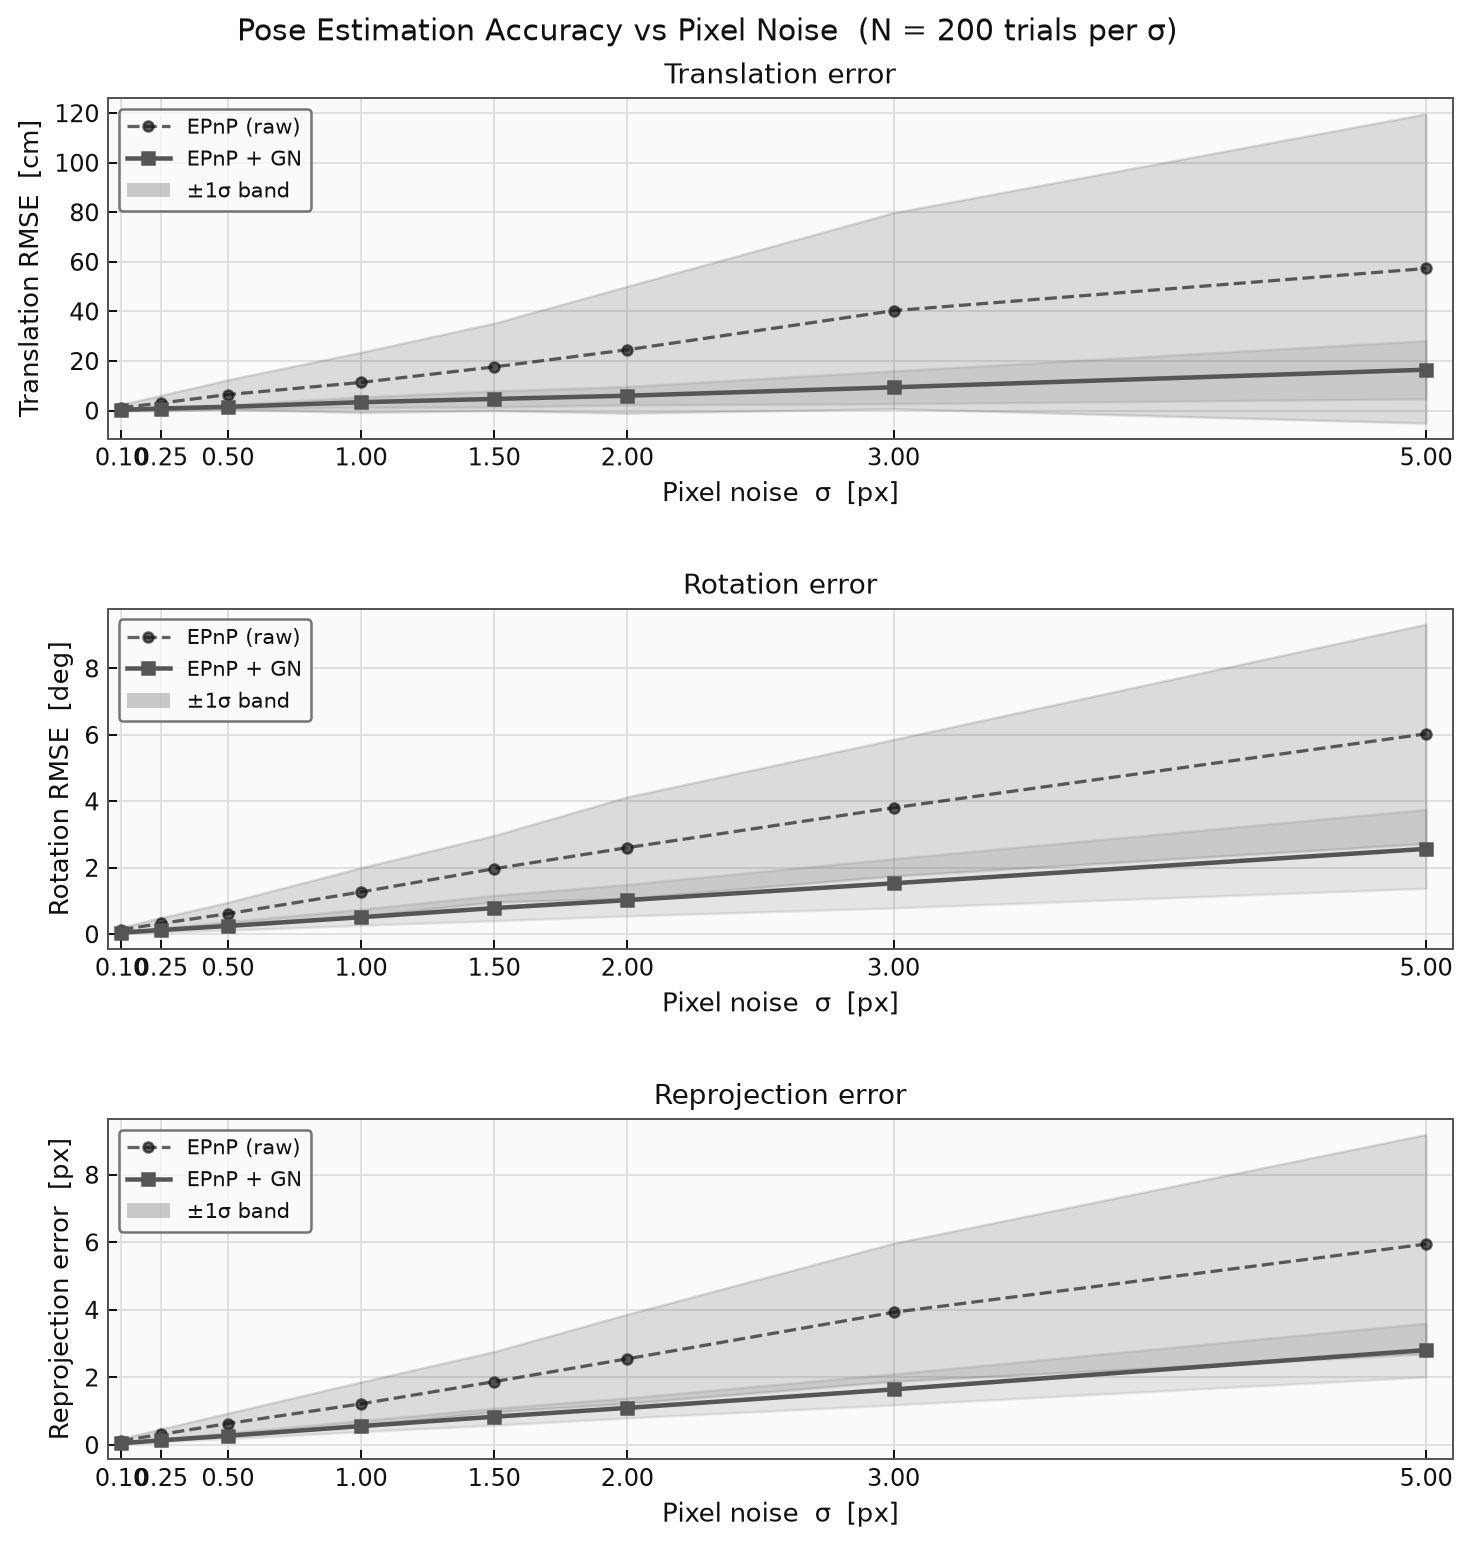
\includegraphics[width=0.86\columnwidth]
    {figures/expB_fig2_pose_vs_noise.png}
    \caption{Pose error against keypoint noise for raw EPnP and after
    Levenberg--Marquardt refinement. 200 trials per level.}
    \label{fig:pose_noise}
\end{figure}

\subsection{Robustness to Correspondence Outliers}
\label{sec:res_ransac}

Table~\ref{tab:ransac} reports the effect of replacing a fraction $f_{out}$ of
the 15 keypoints by uniformly distributed image points, with inlier noise held
at $\sigma_{px} = 1$~px.

\begin{table}[!tb]
\caption{Outlier robustness. 200 trials per level. Errors are RMSE over
successful trials; a dash indicates too few successes to report.}
\label{tab:ransac}
\centering
\begin{tabular}{lrllrll}
\hline
$f_{out}$ & \multicolumn{3}{c}{EPnP alone} & \multicolumn{3}{c}{RANSAC--EPnP} \\
& fail & $t$ [cm] & $\theta$ [$^\circ$] & fail & $t$ [cm] & $\theta$ [$^\circ$] \\
\hline
0\%  & 0\%   & 4.275  & 0.652 & 0\% & 5.175 & 0.854 \\
5\%  & 99\%  & 14.925 & 0.792 & 0\% & 5.364 & 0.842 \\
10\% & 100\% & --     & --    & 0\% & 5.615 & 0.927 \\
20\% & 100\% & --     & --    & 0\% & 6.363 & 0.917 \\
30\% & 100\% & --     & --    & 0\% & 6.074 & 1.037 \\
\hline
\end{tabular}
\end{table}

A single gross outlier destroys the least-squares solution: at
$f_{out} = 5\%$, fewer than one outlier per frame on average, bare EPnP fails
in 99\% of trials. Outlier rejection is not a refinement but a precondition
for applying a PnP solver to real correspondences. RANSAC--EPnP fails in no
trial up to $f_{out} = 30\%$ and degrades only mildly --- 5.18 to 6.07~cm in
translation, 0.854 to 1.037$^\circ$ in attitude --- growth consistent with the
reduced number of true inliers available to the final refit rather than with
any breakdown of the consensus search.

At $f_{out} = 0\%$ RANSAC is slightly \emph{worse} than bare EPnP (5.18~cm
against 4.275~cm). This is expected rather than a defect: the 2~px inlier gate
discards a few legitimate but noisy points, so the final refit uses less data.
Robustness carries a price, and disabling outlier rejection is reasonable when
correspondences are known to be clean.

\begin{figure}[!tb]
    \centering
    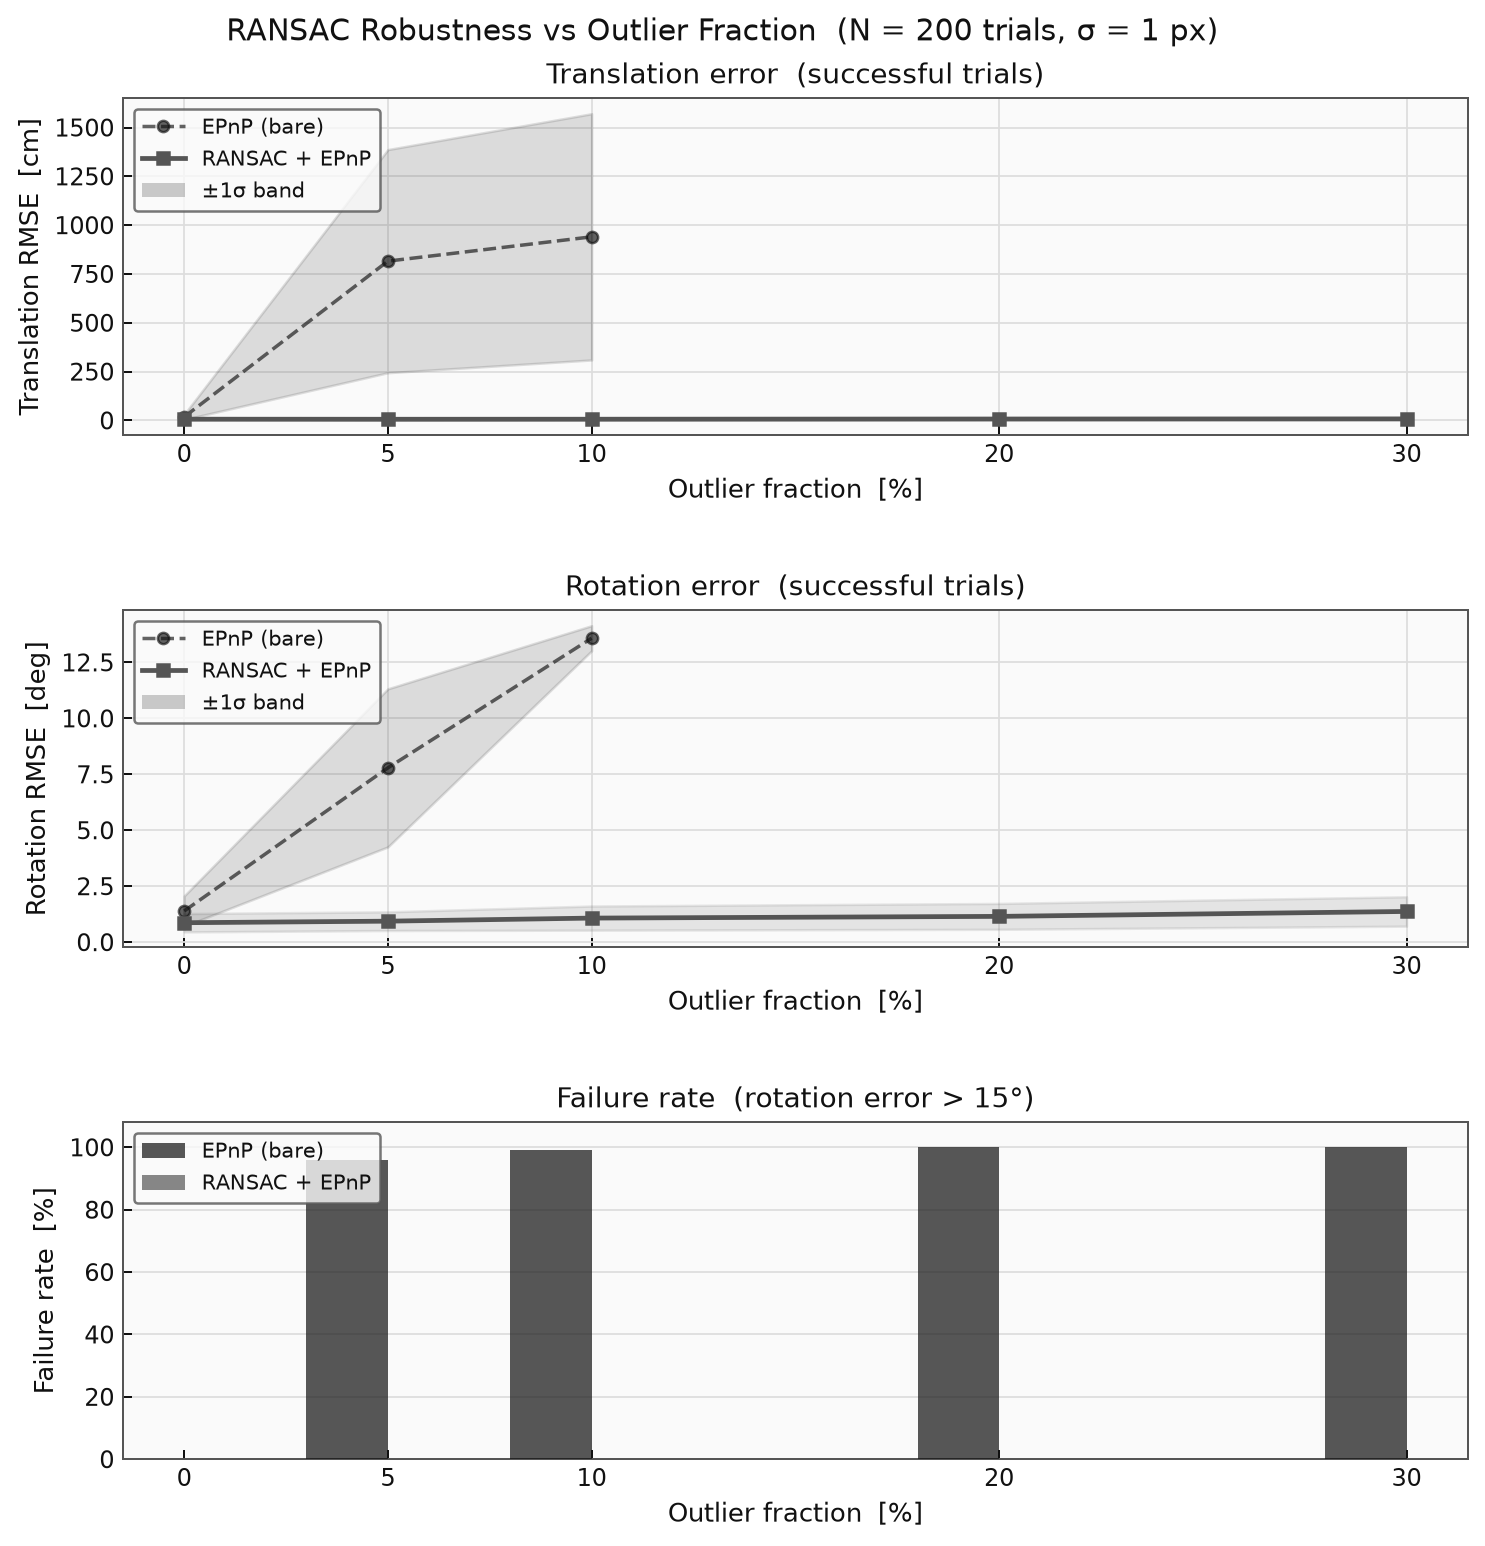
\includegraphics[width=0.86\columnwidth]
    {figures/expC_fig3_ransac_robustness.png}
    \caption{Pose error and failure rate against outlier fraction, for EPnP
    alone and for RANSAC--EPnP. 200 trials per level.}
    \label{fig:ransac_robustness}
\end{figure}

\subsection{Filter Comparison and Consistency}
\label{sec:res_filter}

Experiment~D isolates the estimator: both filters receive an identical
sequence of direct pose measurements over 300 steps, from an initial position
offset of 3.9~m and an initial attitude error of $17^\circ$, with the
perception chain replaced by an equivalent noise model so that filter
behaviour is not confounded with pose-solver failures.

\begin{table}[!tb]
\caption{Multiplicative EKF against UKF on identical measurements. 300 steps,
$\Delta t = 10$~s, seed 42.}
\label{tab:filters}
\centering
\begin{tabular}{lrr}
\hline
Metric & MEKF & UKF \\
\hline
Position RMSE [m]             & 0.5997  & 0.5997 \\
Attitude RMSE [$^\circ$]      & 1.2518  & 1.2802 \\
Velocity RMSE [m/s]           & 0.0226  & 0.0226 \\
Max position error [m]        & 1.5343  & 1.5343 \\
Max attitude error [$^\circ$] & 7.2282  & 7.7671 \\
Measurements accepted         & 300/300 & 300/300 \\
Wall-clock time [s]           & 1.602   & 1.662 \\
\hline
\end{tabular}
\end{table}

The two filters are indistinguishable in translation for a structural rather
than an empirical reason: HCW relative translation is exactly linear, so the
unscented transform and the analytic Jacobian describe the same map and must
agree to machine precision whatever the sigma-point spread. Any difference can
appear only through the attitude and rate block, and there the UKF is
marginally worse, and marginally \emph{slower} --- 1.662~s against 1.602~s,
3.7\% --- as expected of 25 sigma points per step against a single analytic
Jacobian propagation. We therefore find no advantage to the UKF for this
problem and use the MEKF throughout the closed-loop study. Two caveats: the
sigma-point spread parameter must be $O(0.1\text{--}1)$, since with the
frequently quoted $\alpha = 10^{-3}$ and $n_x = 12$ one obtains
$n_x + \lambda = 1.2\times10^{-5}$, a spread of $0.0035\sigma$ and a centre
weight of $-10^{6}$, at which point the unscented transform has collapsed onto
a finite-difference linearisation and an ``EKF versus UKF'' comparison
compares a filter with itself; and these timings are on unpinned consumer
hardware, so the 3.7\% gap should be read as ``no meaningful difference'', not
as a measurement.

Filter consistency is assessed through the normalised innovation squared,
\begin{equation}
\mathrm{NIS}_k = \boldsymbol{\nu}_k^{\top}\mathbf{S}_k^{-1}\boldsymbol{\nu}_k,
\label{eq:nis}
\end{equation}
which for a consistent filter is $\chi^2$ distributed with $n_z = 6$ degrees
of freedom. Over 3600 updates (12 seeds $\times$ 300 steps) the sample mean is
$\bar{\mathrm{NIS}} = 6.044$, against a 95\% confidence interval on the mean of
$[5.887,\,6.113]$ obtained from $n_z \pm 1.96\sqrt{2 n_z / N}$ using
$\mathrm{Var}[\chi^2_k] = 2k$; the fraction of updates exceeding
$\chi^2_{6,0.99} = 16.81$ is 0.97\%, against a nominal 1\%. The filter is
therefore consistent: its reported covariance matches the errors it actually
makes, and the Mahalanobis gate rejects at the designed rate.

This is a stronger statement than a small RMSE, and it rests on three
modelling choices that are easy to get wrong. The attitude residual must be
formed multiplicatively on $SO(3)$ (Sec.~\ref{sec:mekf_residual}); the process
noise must be acceleration-driven with the position--velocity cross terms
retained (Sec.~\ref{sec:process_noise}); and the truth must carry a
disturbance that the filter's $\mathbf{Q}$ actually describes. Substituting a
global rotation-vector residual yields
$\bar{\mathrm{NIS}} = 6.82$, an over-confident filter; removing the truth
disturbance yields 5.77, a conservative one.


\subsection{Guidance: LQR and MPC}
\label{sec:res_control}

Experiment~E compares the infinite-horizon LQR with the receding-horizon MPC
on a 50~m along-track approach, sharing weights, sample time and thrust limit,
with the LQR solution as the MPC terminal cost and the corridor disabled so
that thrust saturation is the only active constraint.


MPC reaches the same terminal accuracy for 5.00~m/s against 16.83~m/s, a 70\%
reduction in propellant. The mechanism must be stated precisely, because the
comparison is easy to over-read. With shared weights and the LQR terminal
cost, an MPC whose constraints are inactive reproduces the infinite-horizon
LQR exactly --- verified here to $4.8\times10^{-7}$. The entire difference is
therefore constraint handling, not prediction: the LQR gain demands
1.77~m/s$^2$ at the initial condition, seventeen times the actuator limit, and
is then clipped per axis, whereas MPC distributes the available authority over
its horizon. The honest framing is \emph{MPC against a saturated LQR}, and the
result is a statement about anti-windup; a constrained-LQR or
reference-governor baseline would narrow the gap and is the appropriate
comparison for future work.

The measured 0.57~ms per step reflects an active-set shortcut: the
corridor-constrained problem is solved only when the corridor is violated at
the box-constrained optimum. With the corridor active throughout, the per-step
cost rises by two orders of magnitude and is dominated by a few hard early
steps, for which a median and 95th percentile are the appropriate statistics.

\begin{figure}[!tb]
    \centering
    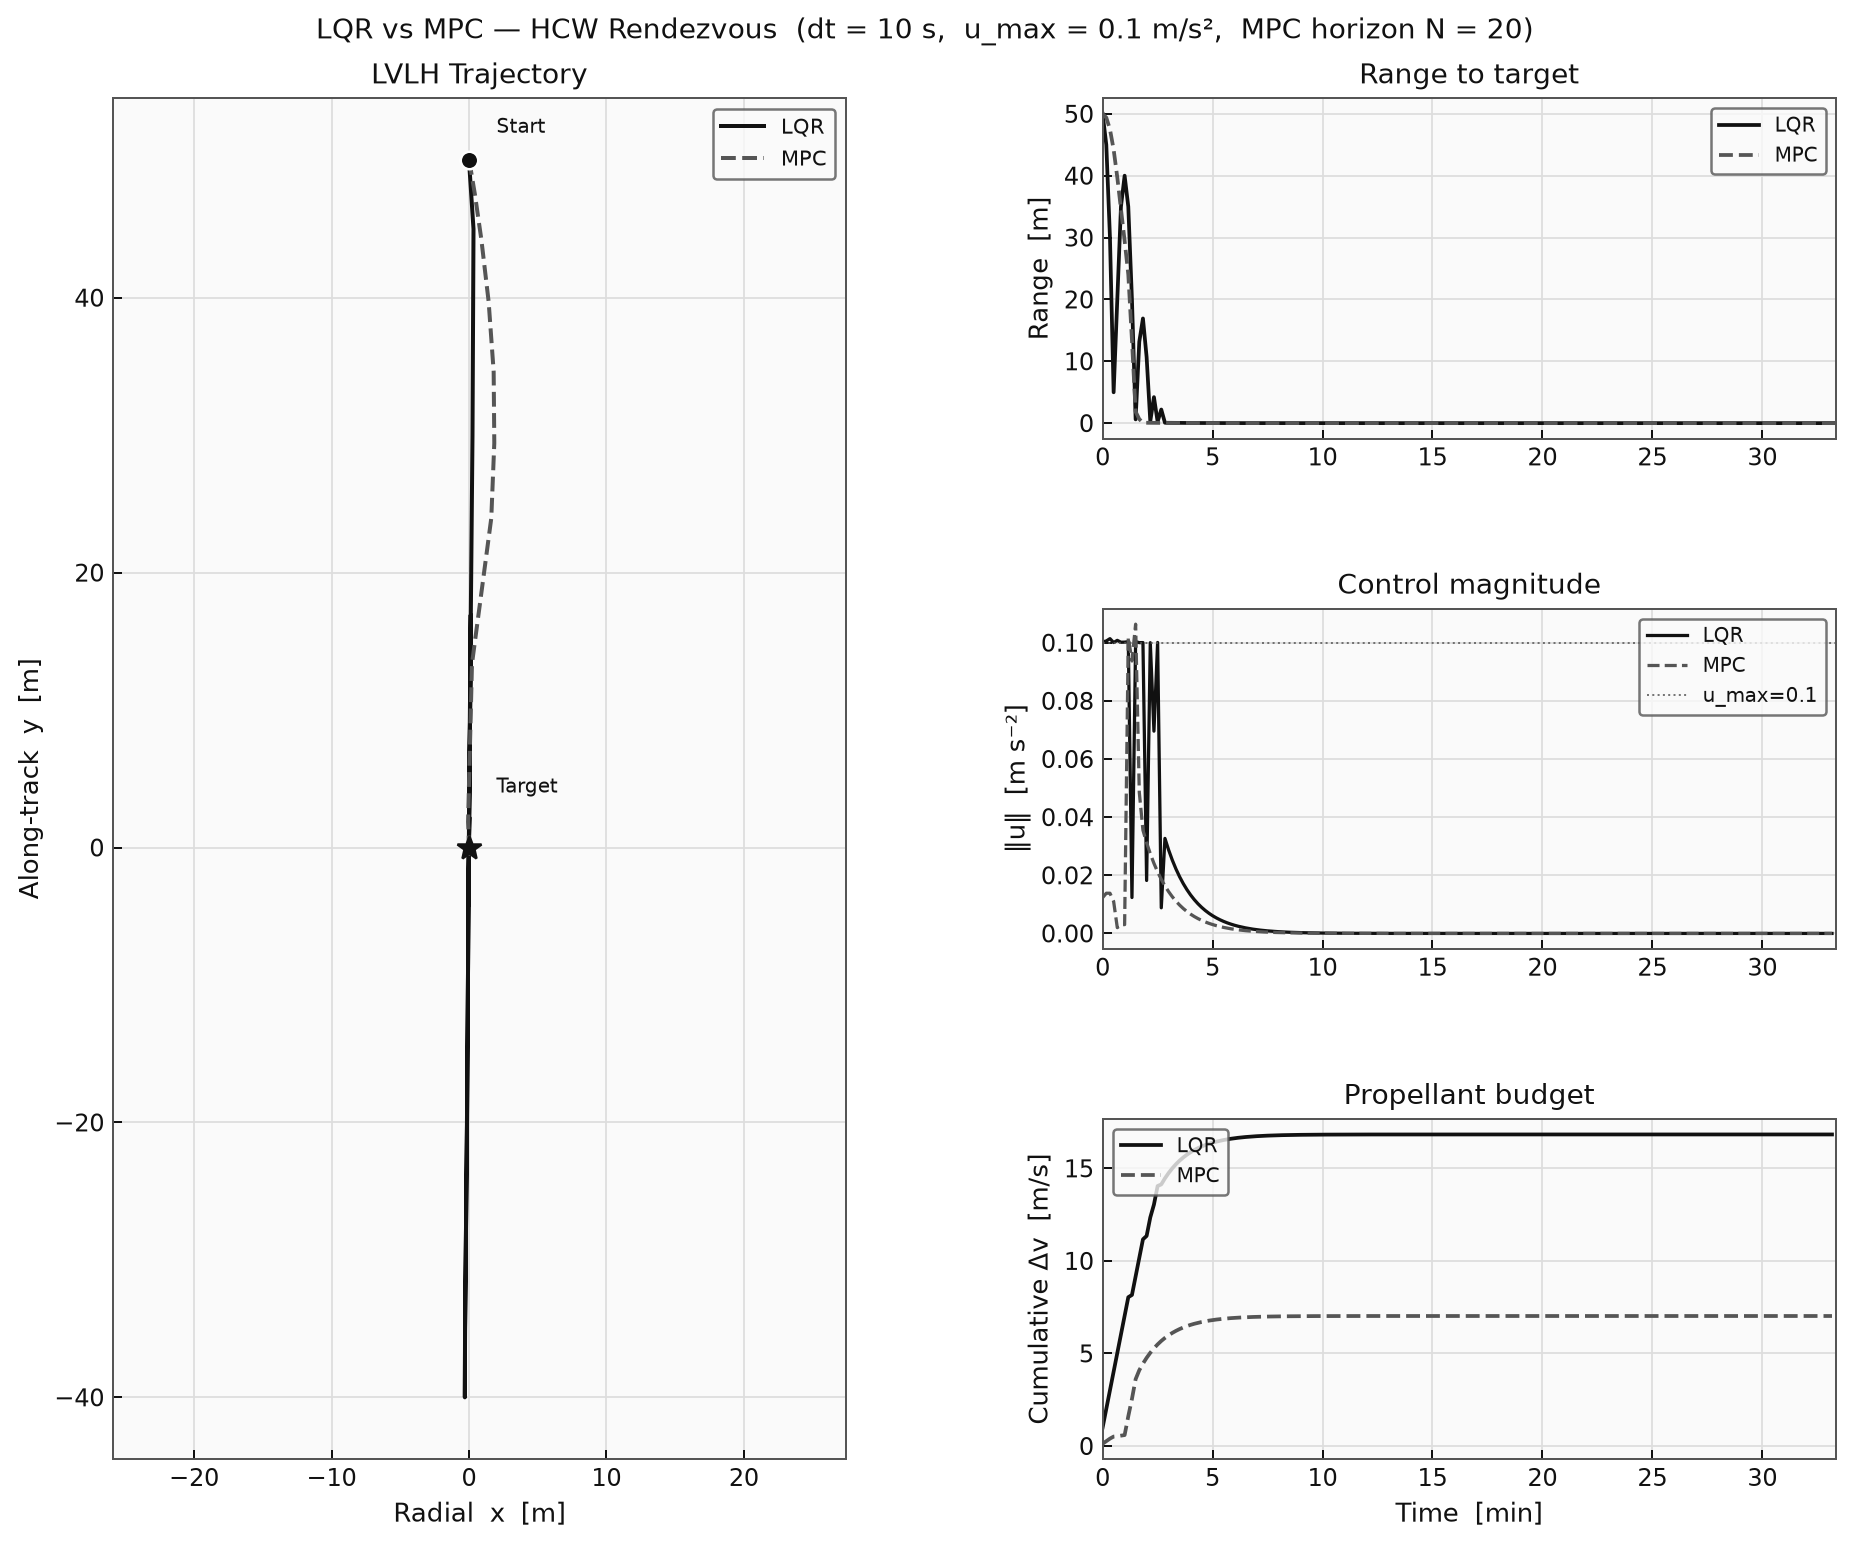
\includegraphics[width=0.86\columnwidth]
    {figures/expE_fig6_lqr_vs_mpc_trajectory.png}
    \caption{LQR and MPC approach trajectories in the LVLH plane.}
    \label{fig:lqr_mpc_traj}
\end{figure}

\subsection{Closed-Loop Performance}
\label{sec:res_closedloop}

The full pipeline was run from a 30~m initial separation with a tumbling
target ($\boldsymbol{\omega}_0 = [0.02,\ 0.05,\ 0.01]$~rad/s).
Table~\ref{tab:closedloop} summarises 12 seeds: all dock, in 2.56~m/s of
$\Delta v$, with no step reaching the thrust limit.

\begin{table}[!tb]
\caption{Closed-loop performance over 12 seeds. Docking is range $<1$~m with
closing speed $<0.05$~m/s.}
\label{tab:closedloop}
\centering
\begin{tabular}{lrr}
\hline
Metric & Mean & Std \\
\hline
Docking step                & 42.7  & 0.6 \\
$\Delta v$ to docking [m/s] & 2.562 & 0.052 \\
Navigation RMSE [m]         & 0.345 & 0.017 \\
Terminal range [m]          & 0.427 & 0.169 \\
Peak closing speed [m/s]    & 1.332 & 0.027 \\
Vision dropout [\%]         & 36.3  & 0.8 \\
Thrust-saturated steps      & 0     & 0 \\
\hline
\end{tabular}
\end{table}

The absence of saturation is a design requirement rather than an
observation: an LQR gain tuned without regard to the actuator limit demands
approximately ninety times $u_{max}$ at 30~m range, saturates on a quarter of
all steps, arrives at 4~m/s and passes through the target before returning ---
a limit cycle rather than a rendezvous. Weighting control so that the
unsaturated demand respects $u_{max}$, and commanding the controller to a
docking-port hold point on the approach axis rather than to the target centre
of mass, reduces the propellant requirement by a factor of sixteen and the
peak closing speed by a factor of three.

\subsection{Measurement Availability as the Limiting Factor}
\label{sec:res_dropout}

The principal finding of the closed-loop study is that the binding constraint
on this architecture is not pose accuracy but \emph{measurement
availability}, and that availability is governed by geometry rather than by
noise.

Availability must be measured against the range the camera is \emph{at}, not
against the range a trial started from. Every trial that closes traverses the
whole range interval, so a trial-level dropout rate averages the far field,
where every keypoint projects inside the frame, with the terminal phase, where
the target overfills the sensor. That rate is accordingly almost constant
across the dispersion:
$34.3\%$, $33.3\%$ and $31.7\%$ for trials beginning in the 10--20~m, 20--30~m
and 30--50~m bands respectively, which says nothing at all.
Table~\ref{tab:dropout} therefore pools the per-step outcome of every step of
every trial in the dispersed campaign of Section~\ref{sec:res_configs} and
bins it by instantaneous range.

\begin{table}[!tb]
\caption{Measurement availability against instantaneous range, pooled over
3887 control steps of 100 dispersed Monte Carlo trials at
$\sigma_{px} = 1.5$~px. A solve is attempted only when at least six keypoints
pass the visibility gate. Intervals are Wilson 95\,\% score intervals on the
per-step availability.}
\label{tab:dropout}
\centering
\begin{tabular}{lrrrr}
\hline
Range [m] & Steps & Mean visible & Availability & 95\,\% CI \\
\hline
10--50   & 1686 & 15.00 & 100.0\% & [99.8,\,100.0] \\
8--10    & 201 & 14.44 & 100.0\% & [98.1,\,100.0] \\
6--8     & 234 & 10.93 & 100.0\% & [98.4,\,100.0] \\
5--6     & 131 &  8.63 &  96.9\% & [92.4,\,98.8] \\
4--5     & 156 &  7.83 &  85.3\% & [78.8,\,90.0] \\
3--4     & 167 &  7.07 &  67.1\% & [59.6,\,73.7] \\
2--3     & 212 &  4.83 &  26.9\% & [21.4,\,33.2] \\
1--2     & 318 &  3.42 &   9.7\% & [7.0,\,13.5] \\
$<1$     & 782 &  2.51 &   1.8\% & [1.1,\,3.0] \\
\hline
\end{tabular}
\end{table}

The profile is a step, not a gradient: availability is statistically
indistinguishable from unity at every range beyond 6~m and falls by a factor
of fifty-five between the 5--6~m and the sub-metre bins.

The mechanism is field-of-view exit, and it is predictable in closed form. A
target of characteristic length $L$ fills a sensor of width $W$ pixels at a
range
\begin{equation}
z_{fill} = \frac{f L}{W},
\label{eq:zfill}
\end{equation}
which for the 8~m Ariane upper stage with $f = 800$~px and $W = 1024$~px gives
$z_{fill} = 6.25$~m. The first bin in Table~\ref{tab:dropout} whose
availability interval excludes unity is 5--6~m, immediately inside that
prediction. Inside $z_{fill}$ the number of keypoints simultaneously within the
image falls below the six required for a minimal RANSAC sample --- the mean
visible count crosses six between the 4--5~m and 3--4~m bins --- and the pose
solution becomes unavailable regardless of detector accuracy.

This has a direct consequence for the noise ablation.
Table~\ref{tab:ablation} sweeps $\sigma_{px}$ over 40 dispersed trials per
level, \emph{paired}: the same seed sequence generates the initial position,
velocity, tumble rate and attitude at every noise level, so the level-to-level
difference is the effect of the parameter and not of a fresh draw of initial
conditions.

\begin{table}[!tb]
\caption{Terminal accuracy and docking success against keypoint noise. 40
dispersed trials per level, paired across levels, full vision--MEKF pipeline.
Terminal range is reported as the median with 5th and 95th percentiles: a
single diverging trial dominates the mean and its standard deviation.
Docking intervals are Wilson 95\,\% score intervals.}
\label{tab:ablation}
\centering
\begin{tabular}{lrrr}
\hline
$\sigma_{px}$ [px] & Terminal range [m] & Docking & 95\,\% CI \\
\hline
0.3 & 0.34 [0.11,\,0.78]  & 100\% & [91,\,100] \\
0.7 & 0.33 [0.14,\,0.82]  & 100\% & [91,\,100] \\
1.0 & 0.32 [0.11,\,0.81]  & 100\% & [91,\,100] \\
1.5 & 0.30 [0.13,\,0.82]  & 100\% & [91,\,100] \\
2.0 & 0.32 [0.09,\,0.73]  &  98\% & [87,\,100] \\
3.0 & 0.34 [0.15,\,8.22]  &  95\% & [83,\,99]  \\
4.0 & 0.51 [0.17,\,12.47] &  85\% & [71,\,93]  \\
\hline
\end{tabular}
\end{table}

The median terminal range is flat from 0.3 to 3.0~px --- it varies by 4~cm
while the noise grows tenfold --- and the degradation appears first in the
\emph{tail}, not in the centre of the distribution. The 95th percentile rises
from 0.73~m at 2~px to 8.22~m at 3~px and 12.47~m at 4~px, and docking success
falls from $100\%$ to $85\%$ over the same interval. The median trial at 4~px
docks as tightly as the median trial at 0.3~px while roughly one trial in
seven diverges completely: the signature of a threshold, not of drift. The
threshold is the point at which the pose solver's success rate inside $z_{fill}$ falls low
enough that the filter coasts on prediction for the whole terminal phase, and
the accumulated dead-reckoning error exceeds the docking corridor before the
range gate is satisfied.

The dispersion also weakens a conclusion that a single-trajectory study would
have supported. Repeating this ablation along one fixed approach trajectory,
varying only the noise realisation, yields a far sharper collapse --- 65\%
success at 4~px with a terminal-range standard deviation above 100~m ---
because every trial then encounters the field-of-view knee at the same
geometry and the same phase of the tumble. Dispersing the initial condition
spreads that encounter, and the honest statement of the effect is the milder
one in Table~\ref{tab:ablation}. We report both because the difference is
itself the argument for dispersing: a Monte Carlo campaign that varies only
the random seed measures the repeatability of one trajectory, not the
robustness of a design.

Two implications follow. First, the useful figure of merit for a monocular
front end in this role is not pose RMSE but the probability of returning a
usable solution, and the two do not degrade together: between 0.3 and 2.0~px
the pose error grows by a factor of seven (Table~\ref{tab:pose_noise}) while
closed-loop performance is unchanged. Second, terminal approach inside
$z_{fill}$ requires a change of sensing modality --- a wider lens, a second
short-range camera, or a close-range keypoint subset chosen to remain in
frame --- and no improvement in the pose solver will substitute for it. The
design margin worth buying is field of view and keypoint redundancy at short
range, not sub-pixel feature localisation.

\begin{figure}[!tb]
    \centering
    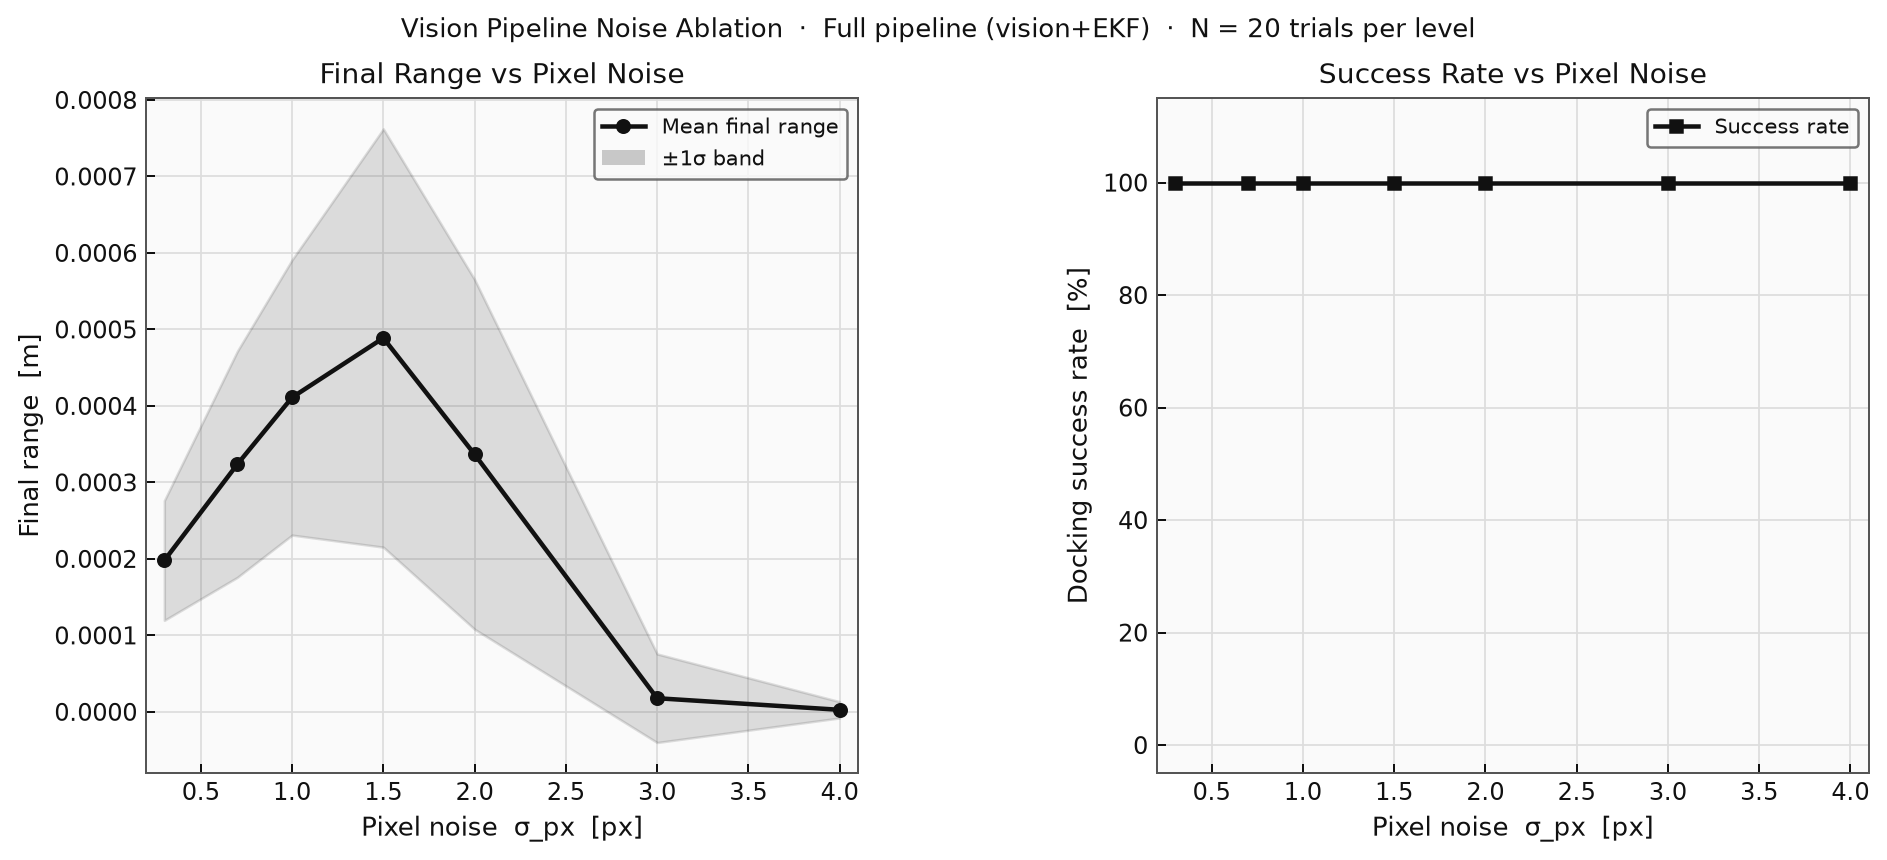
\includegraphics[width=0.86\columnwidth]
    {figures/expF_fig9_ablation_noise.png}
    \caption{Terminal range, docking success and vision dropout against
    keypoint noise, 40 paired dispersed trials per level. The envelope is flat
    to 2~px; the degradation beyond it appears in the tail of the terminal
    range distribution while the median is unchanged.}
    \label{fig:ablation}
\end{figure}

\begin{figure}[!tb]
    \centering
    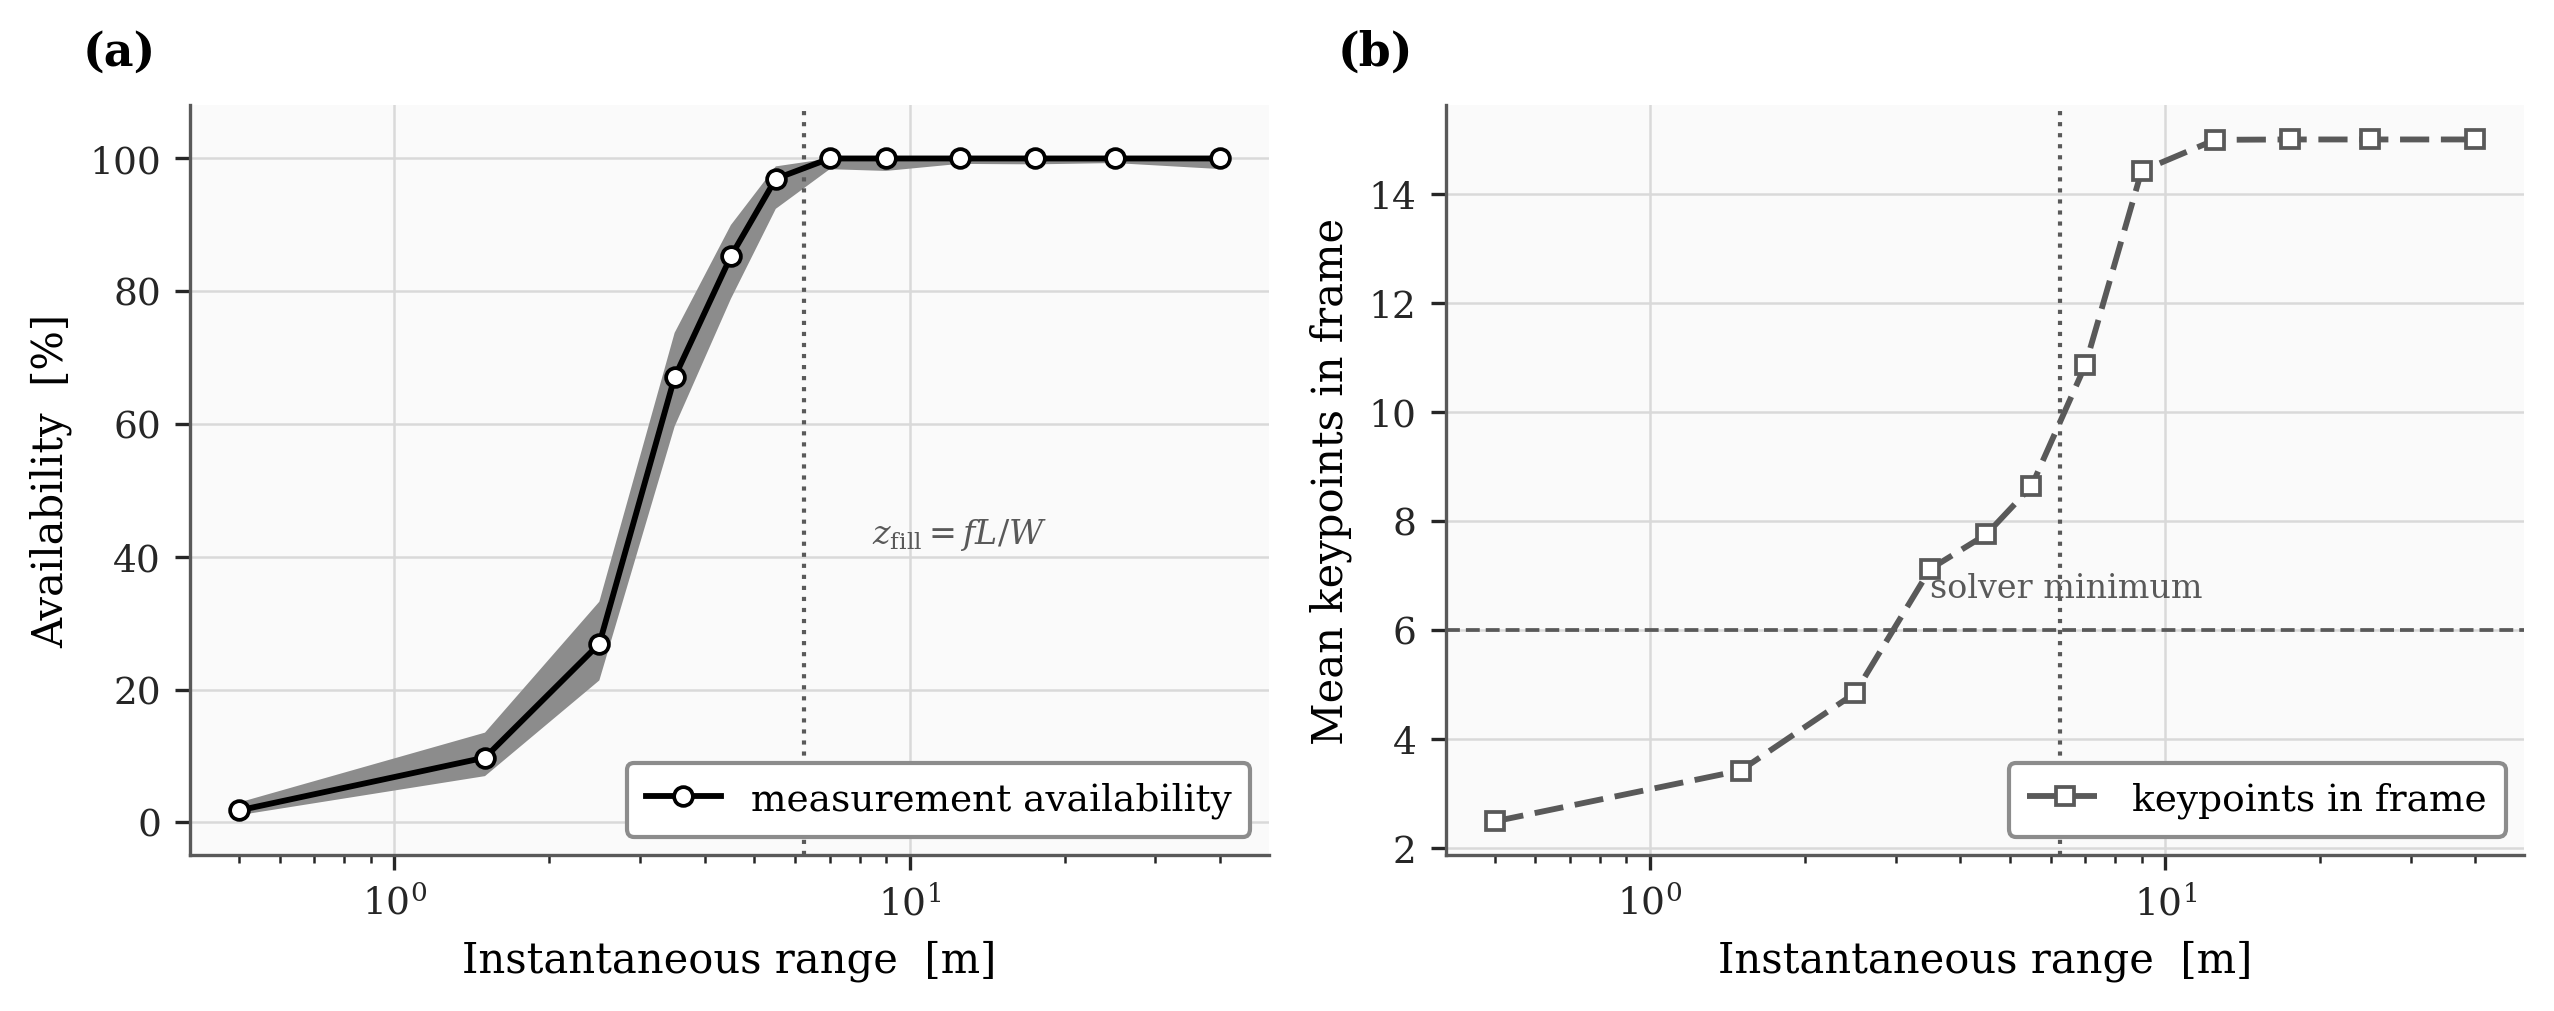
\includegraphics[width=0.86\columnwidth]
    {figures/expF_fig10_availability.png}
    \caption{(a) Per-step measurement availability against instantaneous
    range, pooled over the 100-trial dispersed campaign, with the closed-form
    fill range $z_{fill} = fL/W = 6.25$~m marked. Shading is the Wilson
    95\,\% interval. (b) Mean number of keypoints passing the visibility gate;
    the six-keypoint solver minimum is crossed just inside $z_{fill}$.}
    \label{fig:availability}
\end{figure}

\subsection{Dispersed Monte Carlo Campaign}
\label{sec:res_configs}

The configurations are compared over a dispersed Monte Carlo campaign rather
than over repeated runs of one trajectory. Each trial draws an initial range log-uniformly on $[15, 45]$~m, a bearing uniformly within a
$20^{\circ}$ cone about the radial approach axis, a closing speed uniformly on
$[-0.15, -0.02]$~m/s with a $1\,\mathrm{cm/s}$ transverse component, a tumble
rate uniformly on $[0.005, 0.09]$~rad/s about an isotropically distributed
axis, an initial target attitude uniform on $SO(3)$ by Shoemake's method, and
a navigation initialisation error of $1.5$~m and $2$~cm/s per axis
$(1\sigma)$. Trials are seeded from a single \texttt{SeedSequence}, spawned
per trial and split again into an independent dispersion stream and simulator
stream, so any trial is reproducible in isolation, is independent of the
campaign size and of execution order, and is identical whether the campaign
runs serially or in parallel. The three configurations share that seed
sequence and are therefore compared trial-by-trial on identical initial
conditions.

\begin{table}[!tb]
\caption{Configuration comparison over 100 dispersed trials each, paired
across configurations, $\sigma_{px} = 1.5$~px where applicable. Terminal range
is the median with 5th and 95th percentiles; docking intervals are Wilson
95\,\% score intervals.}
\label{tab:configs}
\centering
\begin{tabular}{lrrr}
\hline
Configuration & Range [m] & $\Delta v$ [m/s] & Docking \\
\hline
Perfect state             & 0.33 & $2.53 \pm 0.80$ & 100\% [96,\,100] \\
Direct measurement + MEKF & 0.54 & $2.65 \pm 0.81$ & 100\% [96,\,100] \\
Full vision + MEKF        & 0.33 & $2.52 \pm 0.80$ & 100\% [96,\,100] \\
\hline
\end{tabular}
\end{table}

The three configurations lie within 5\% of one another in propellant and dock
in every one of the 300 trials. We draw a deliberately narrow conclusion: at
$\sigma_{px} = 1.5$~px the perception chain is \emph{not} the limiting
subsystem, and closed-loop performance is set by the guidance law and the
actuator limit. It would be a mistake to read the full pipeline's marginal
advantage over the direct-measurement baseline as evidence that vision
outperforms a half-metre position sensor: the two configurations have
different measurement error magnitudes, and the comparison is informative only
about which subsystem is binding --- which at this noise level is neither. It
becomes discriminating only above 3~px, where Table~\ref{tab:ablation} shows
the perception chain taking over as the limiting factor.

Two aspects of the campaign design are worth stating explicitly, because both
were defects in an earlier version of this study. First, the perfect-state
configuration has no sensor noise anywhere, so if only the random seed were
varied its trials would be bit-identical and its reported distribution would
be an artefact; dispersing the initial condition gives it a genuine
distribution, and the $\Delta v$ spread of $\pm 0.80$~m/s in
Table~\ref{tab:configs} is the spread induced by the initial condition alone,
which is the correct baseline against which to read the other two rows.
Second, mean $\Delta v$ over all trials is not a propellant budget when some
trials fail, so the campaign reports it conditioned on docking as well; here
the two coincide because every trial docked, but they diverge in the ablation
of Table~\ref{tab:ablation}.


\section{Conclusion}

This paper presented a modular closed-loop simulation framework
for vision-based autonomous spacecraft rendezvous and evaluated
each component of the perception, estimation, and guidance
pipeline through six targeted experiments.

The dynamics experiment confirmed that the HCW state-transition
implementation is numerically consistent with high-accuracy DOP853
integration to sub-nanometer position precision over three orbital
periods, validating the dynamics model as a suitable foundation
for the subsequent control and estimation studies.

The pose-estimation experiments established two complementary
properties of the visual pipeline.
First, Gauss--Newton nonlinear refinement substantially reduces
the raw EPnP translation error across all tested noise levels,
achieving a $76\%$ reduction at $5$~px pixel noise.
Second, RANSAC-based correspondence rejection is essential for
robustness: bare EPnP failed in up to $100\%$ of trials at
$30\%$ outlier contamination, while RANSAC--EPnP maintained
zero solver failures and sub-$8$~cm translation accuracy
throughout the tested range.

The state-estimation comparison showed that MEKF and UKF achieve
effectively identical translational performance under the
controlled Gaussian measurement model, with position and
velocity RMSE of $0.60$~m and $0.023$~m/s respectively.
The MEKF produced a marginally lower attitude RMSE
($1.33^\circ$ vs $1.34^\circ$), while the UKF required
approximately half the wall-clock execution time.

The guidance and control experiment revealed a clear performance
trade-off between the two strategies.
MPC achieved $58\%$ lower cumulative $\Delta v$ than LQR
($7.02$~m/s vs $16.83$~m/s) for the same rendezvous task,
but at a $300\times$ higher per-step computational cost
($3.00$~ms vs $0.01$~ms).
Both controllers converged to sub-millimetre final range,
confirming that terminal accuracy is not a differentiating factor
for the unconstrained scenario evaluated here.

The end-to-end Monte Carlo study demonstrated $100\%$ docking
success over 25 trials for all three configurations tested:
perfect-state feedback, direct noisy-measurement EKF, and the
full vision--MEKF pipeline.
The full pipeline achieved cumulative $\Delta v$ comparable to
the perfect-state reference ($\approx40.2$~m/s), substantially
below the direct EKF configuration ($\approx68.2$~m/s), showing
that RANSAC--EPnP visual measurements provide cleaner state
estimates than direct noisy position measurements under the
tested conditions.
The pixel-noise ablation further confirmed that $100\%$ docking
success is maintained from $0.3$~px to $4.0$~px, demonstrating
substantial tolerance of the closed-loop system to image-plane
measurement degradation.

Taken together, the results validate the proposed architecture
at both the subsystem and system level.
The principal limitation of the present study is its reliance on
a simplified synthetic camera model with parametric keypoints
and additive Gaussian noise; real imagery introduces
illumination variation, partial target visibility,
texture-dependent matching ambiguities, and hardware-specific
noise characteristics not captured by this model.

Future work should address these limitations through integration
of a higher-fidelity rendering pipeline, extension to
unstructured natural-feature keypoints, and hardware-in-the-loop
testing with a real camera and representative embedded processor.
Incorporating $J_2$ and atmospheric drag perturbations into
the dynamics model and evaluating the MPC approach-cone constraint
in the closed-loop end-to-end pipeline are also important
directions for future investigation.


% -------------------------------------------------
% References
% -------------------------------------------------

\bibliographystyle{IEEEtran}
\bibliography{references}

\end{document}